\section{Alignment}
\label{sec:Alignment}

Several cross checks have been performed in order to ensure the telescope and the DUT are correctly aligned.

\subsection{Rotations around the $z$ axis}

Potential rotations of the DUT around the $z$ axis have been studied by looking at the $x$ residuals as a function of the $y$ position. If the DUT is properly aligned, the $x$ residuals are expected to be independent of the $y$ position, while a rotation of the DUT around the $z$ axis would manifest itself as a linear dependence between the two variables.
Two examples, corresponding to a good and a bad alignment, are shown on the left and, respectively, on the right of Fig. \ref{fig:RotationZ}.
A straight line fit has been performed for each measurement taken at the nominal angle around the $y$ axis. The mean of the angular coefficient distribution has then  been used to correct for the misalignment when determining the extrapolated position of the track on the DUT plane. The distributions of the intercept $a_0$ and the angular coefficient $a_1$, obtained for the M1 board with the fan-in pitch adapter, are shown as reference in Fig. \ref{fig:CheckZRot}.

\begin{figure}[]
\centering
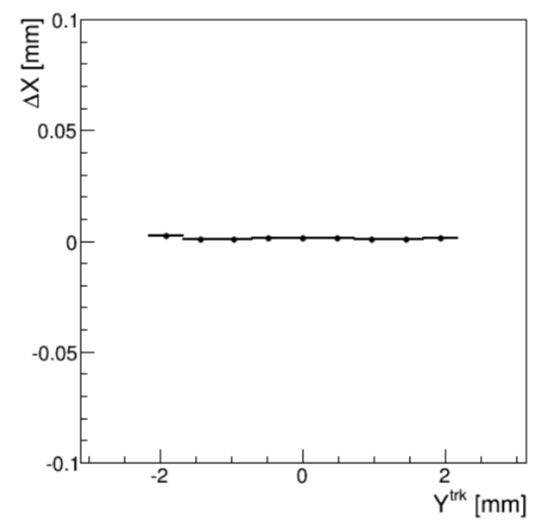
\includegraphics[width=0.45\textwidth]{figs/RotationZGood.png}
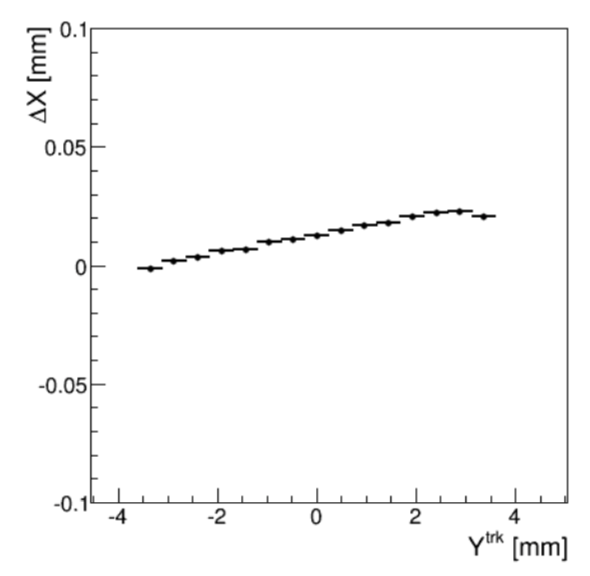
\includegraphics[width=0.45\textwidth]{figs/RotationZBad.png}
\caption[Examples of $x$ residuals as a function of the $y$ position.]{Examples of $x$ residuals as a function of the $y$ position for a DUT that is properly aligned (left) and for a DUT that is rotated around the $z$ axis (right).}
\label{fig:RotationZ}
\end{figure}

\begin{figure}[]
\centering
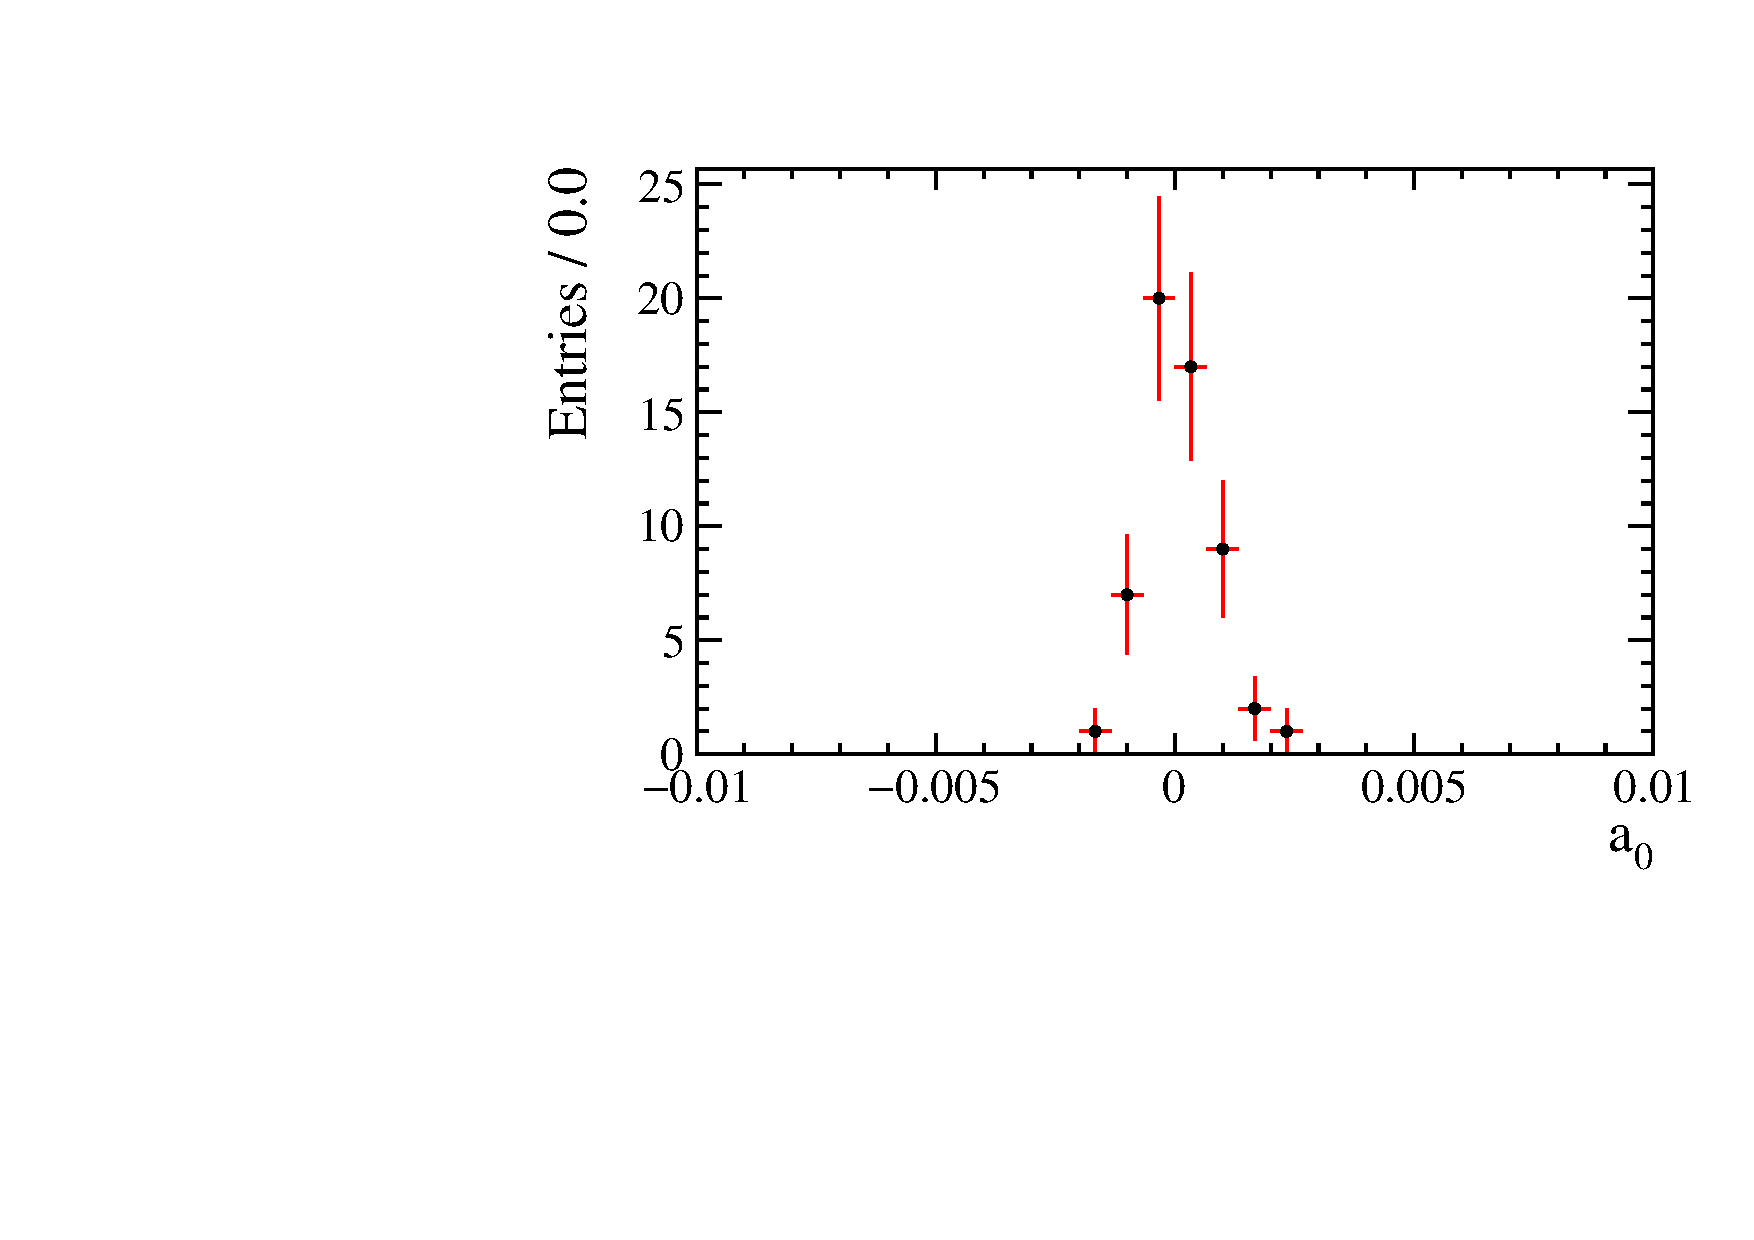
\includegraphics[width=0.45\textwidth]{figs/CheckZRot/ca0_M1_FanIn.pdf}
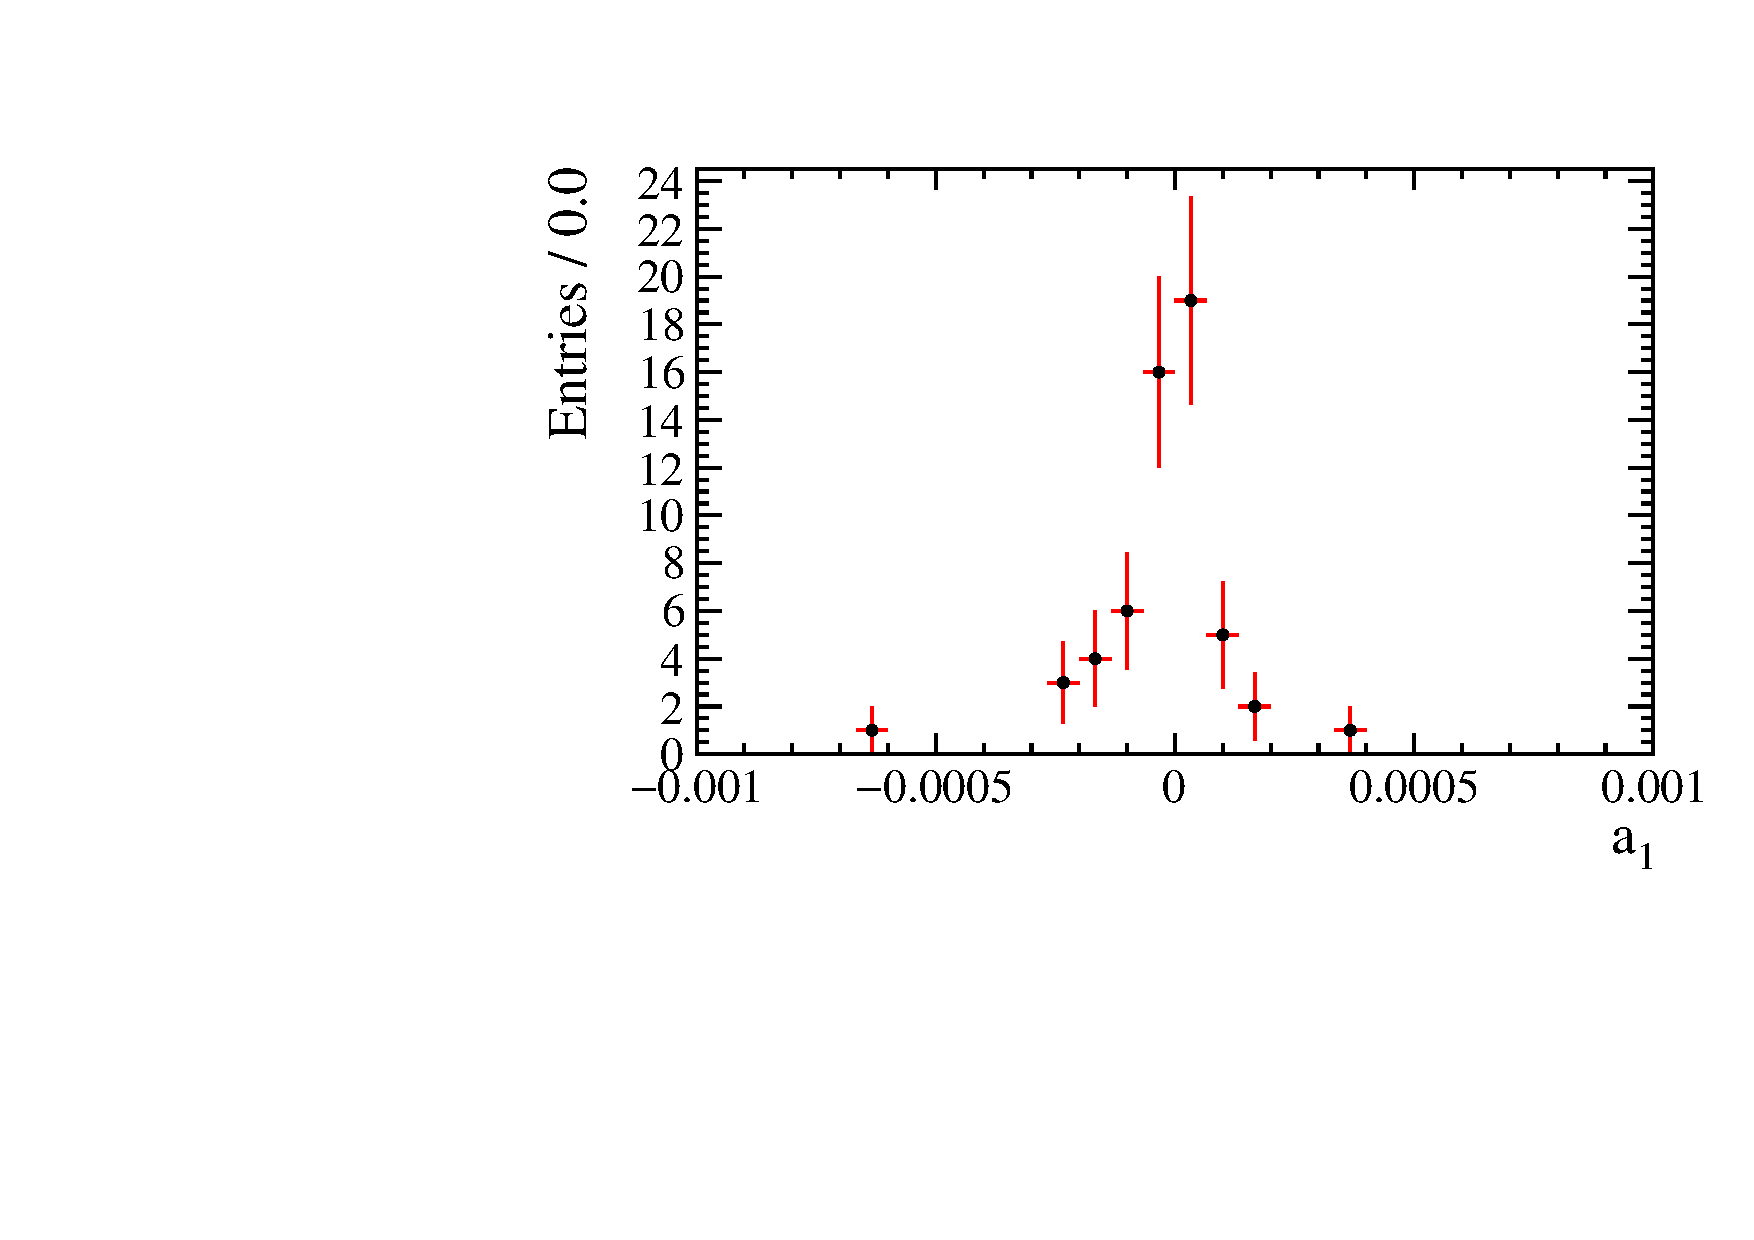
\includegraphics[width=0.45\textwidth]{figs/CheckZRot/ca1_M1_FanIn.pdf}
\caption[Distributions of the intercept $a_0$ and the angular coefficient $a_1$.]{Distributions of the intercept $a_0$ (left) and the angular coefficient $a_1$ (right), obtained for the M1 board with the fan-in pitch adapter.}
\label{fig:CheckZRot}
\end{figure}

An alternative method to check the same kind of misalignment consists in studying the charge sharing as a function of the cluster interstrip position for different rotations around the $y$ axis. The charge sharing is here defined as
\begin{displaymath}
\eta = \frac{Q_R}{Q_L+Q_R},
\end{displaymath}
that is, as the fraction of total charge deposited on the right strip.
The cluster interstrip position is defined as the distance, in units of strip pitch, from the point in between two adjacent strips.
According to these definitions, the charge sharing varies between $0$ and $1$, while the cluster interstrip position has values between $-0.5$ and $0.5$.
The dependence of the charge sharing as a function of the cluster interstrip position on the rotation around the $y$ axis is shown in Fig. \ref{fig:ChargeSharingvsAngle} for the M3 fan-up sensor with top biasing. Similar plots are available for the other sensors.
Each distribution in Fig. \ref{fig:ChargeSharingvsAngle} has been fitted with an error function of the form
\begin{displaymath}
...
\end{displaymath}
The fit results are shown in Table \ref{tab:ErrorFunctions}.
The $\mu$ as a function of the angle around the $y$ axis...
The $\sigma$ as a function of the angle of rotation around the $y$ axis is expected to have a minimum at zero degrees and to be symmetrically distributed around the minimum.
The dependence of the parameters $\mu$ and $\sigma$ on the rotation around the $y$ axis is shown in Fig. \ref{fig:ChargeSharingvsAngle2}.

\begin{figure}[]
\centering
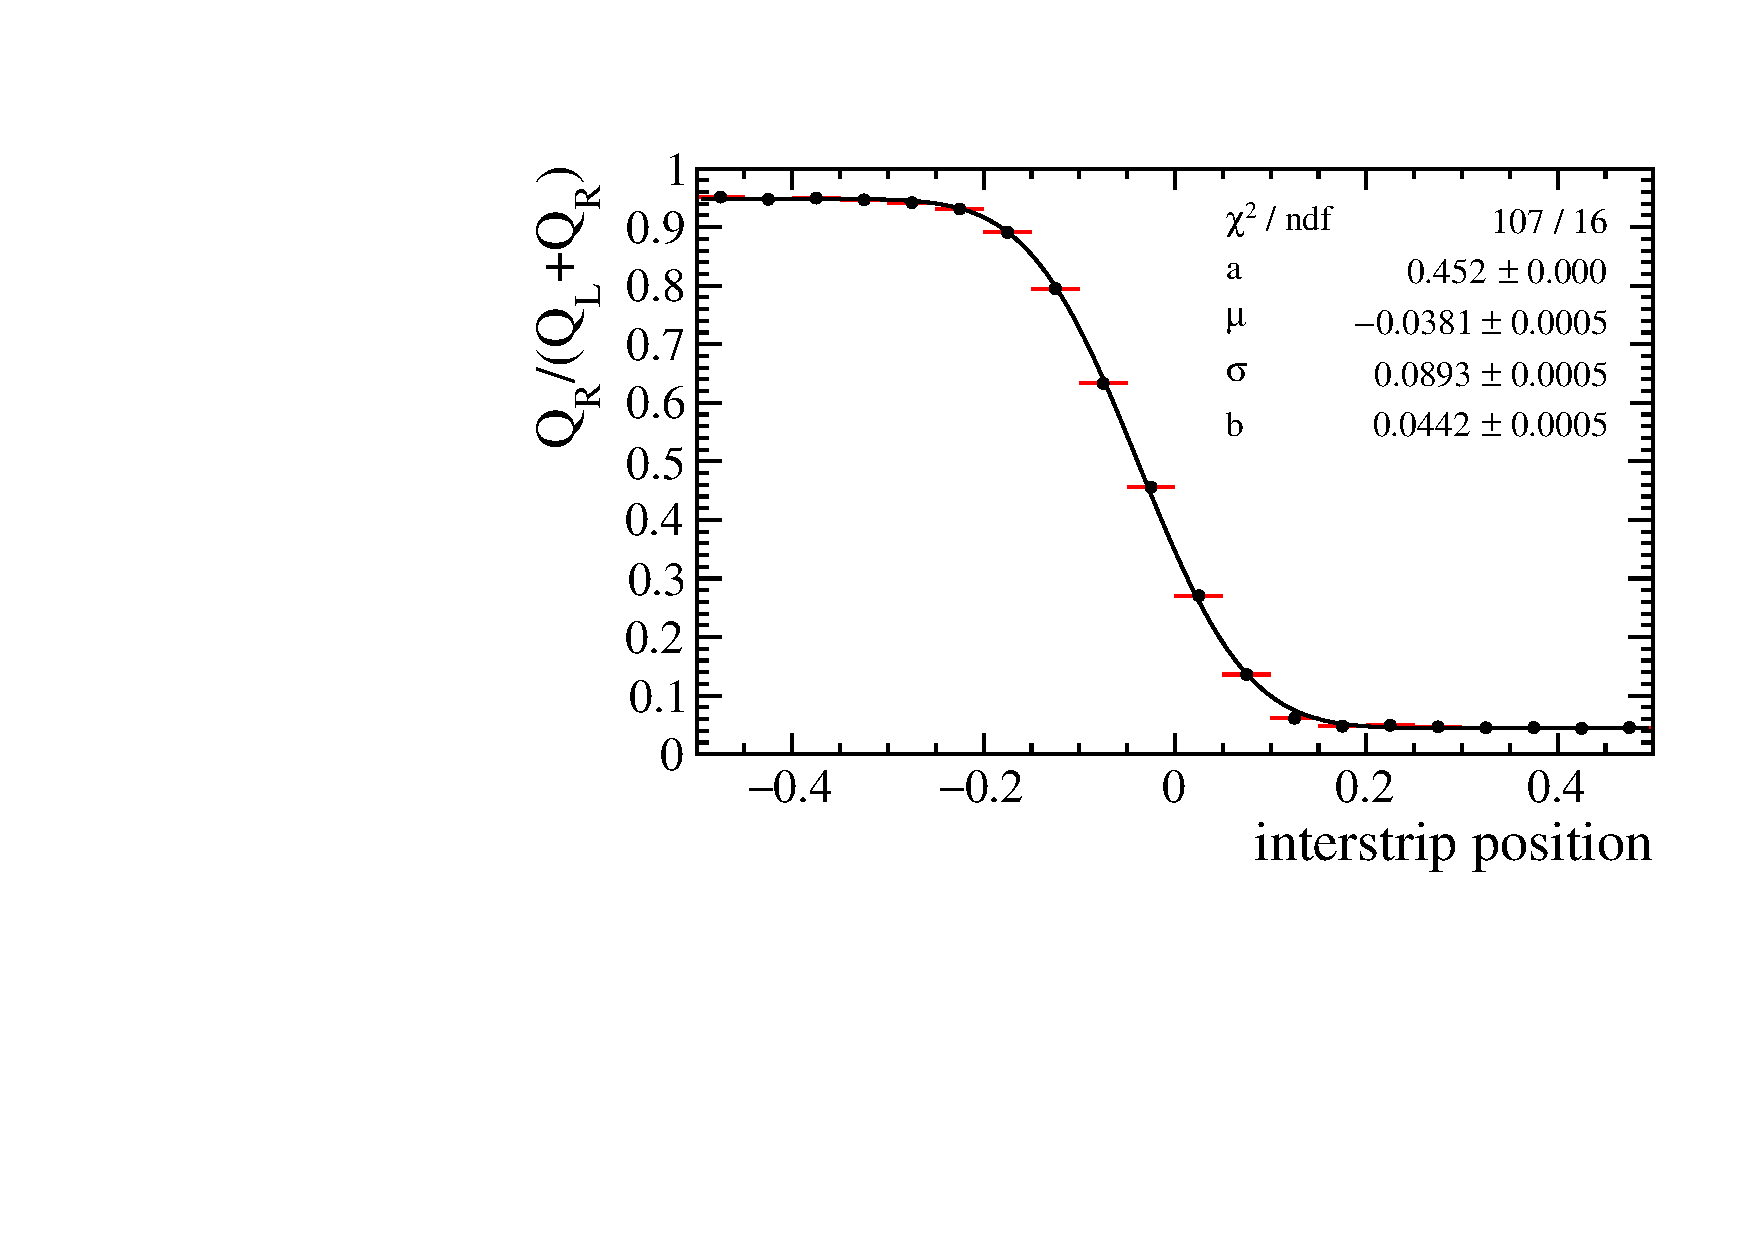
\includegraphics[width=0.4\textwidth]{figs/ChargeSharingvsAngle/cchargeSharing_M3_FanUp_Top_-10.pdf}
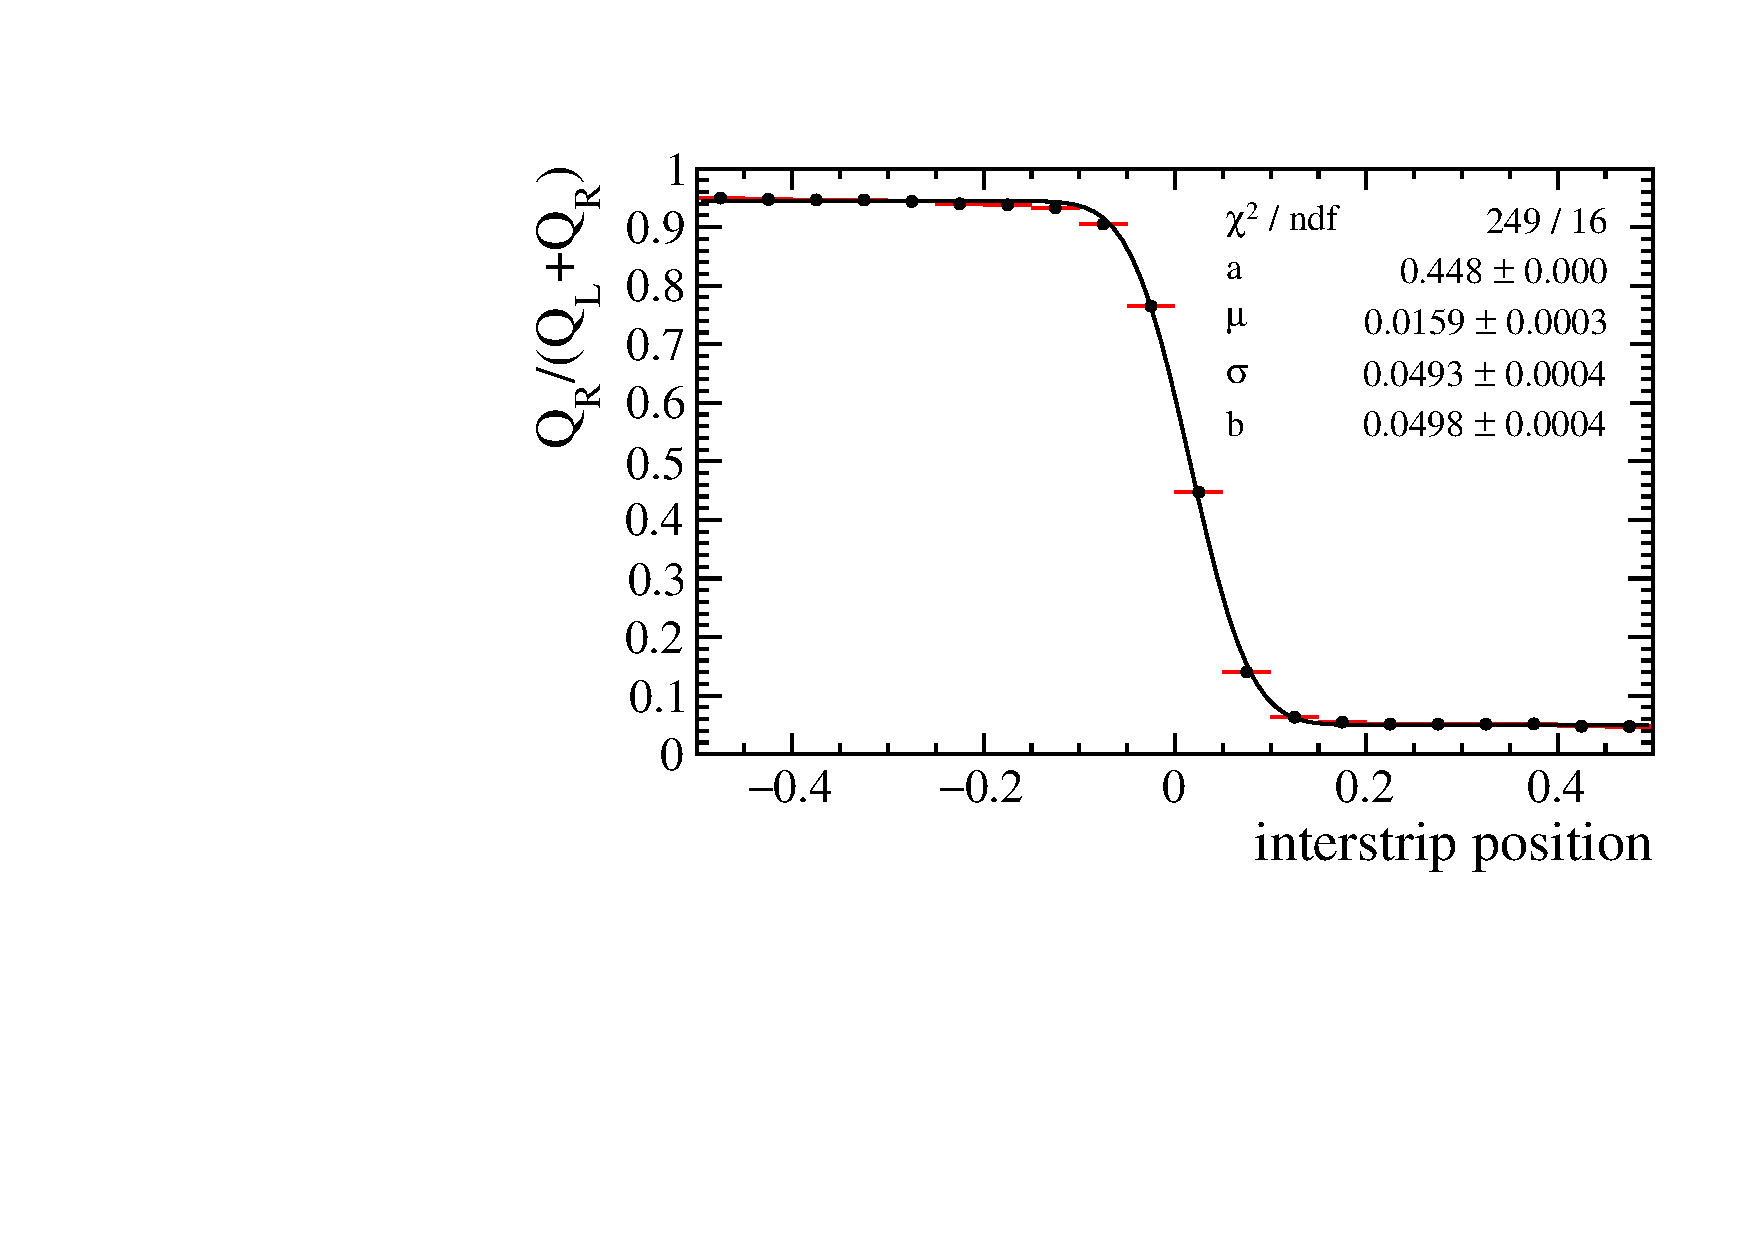
\includegraphics[width=0.4\textwidth]{figs/ChargeSharingvsAngle/cchargeSharing_M3_FanUp_Top_-5.pdf}
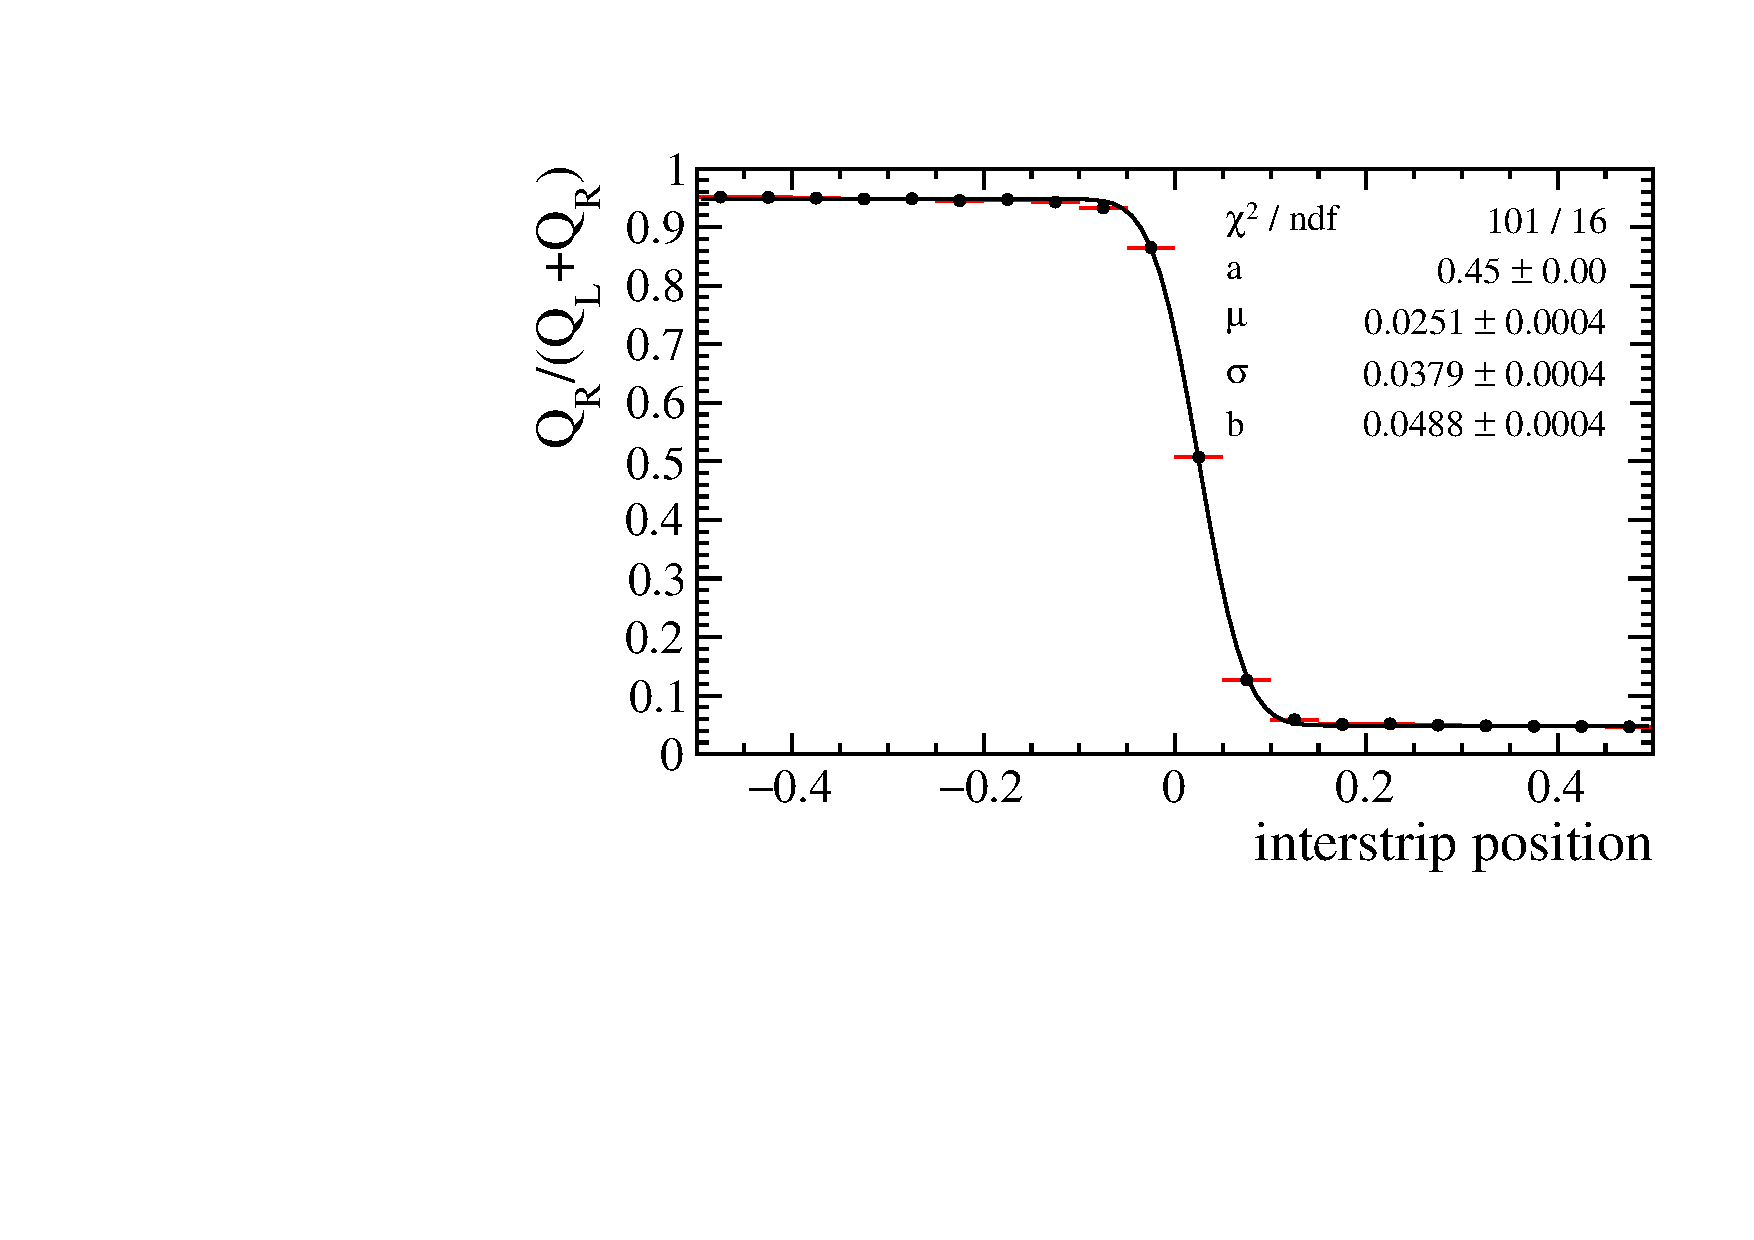
\includegraphics[width=0.4\textwidth]{figs/ChargeSharingvsAngle/cchargeSharing_M3_FanUp_Top_-2.pdf}
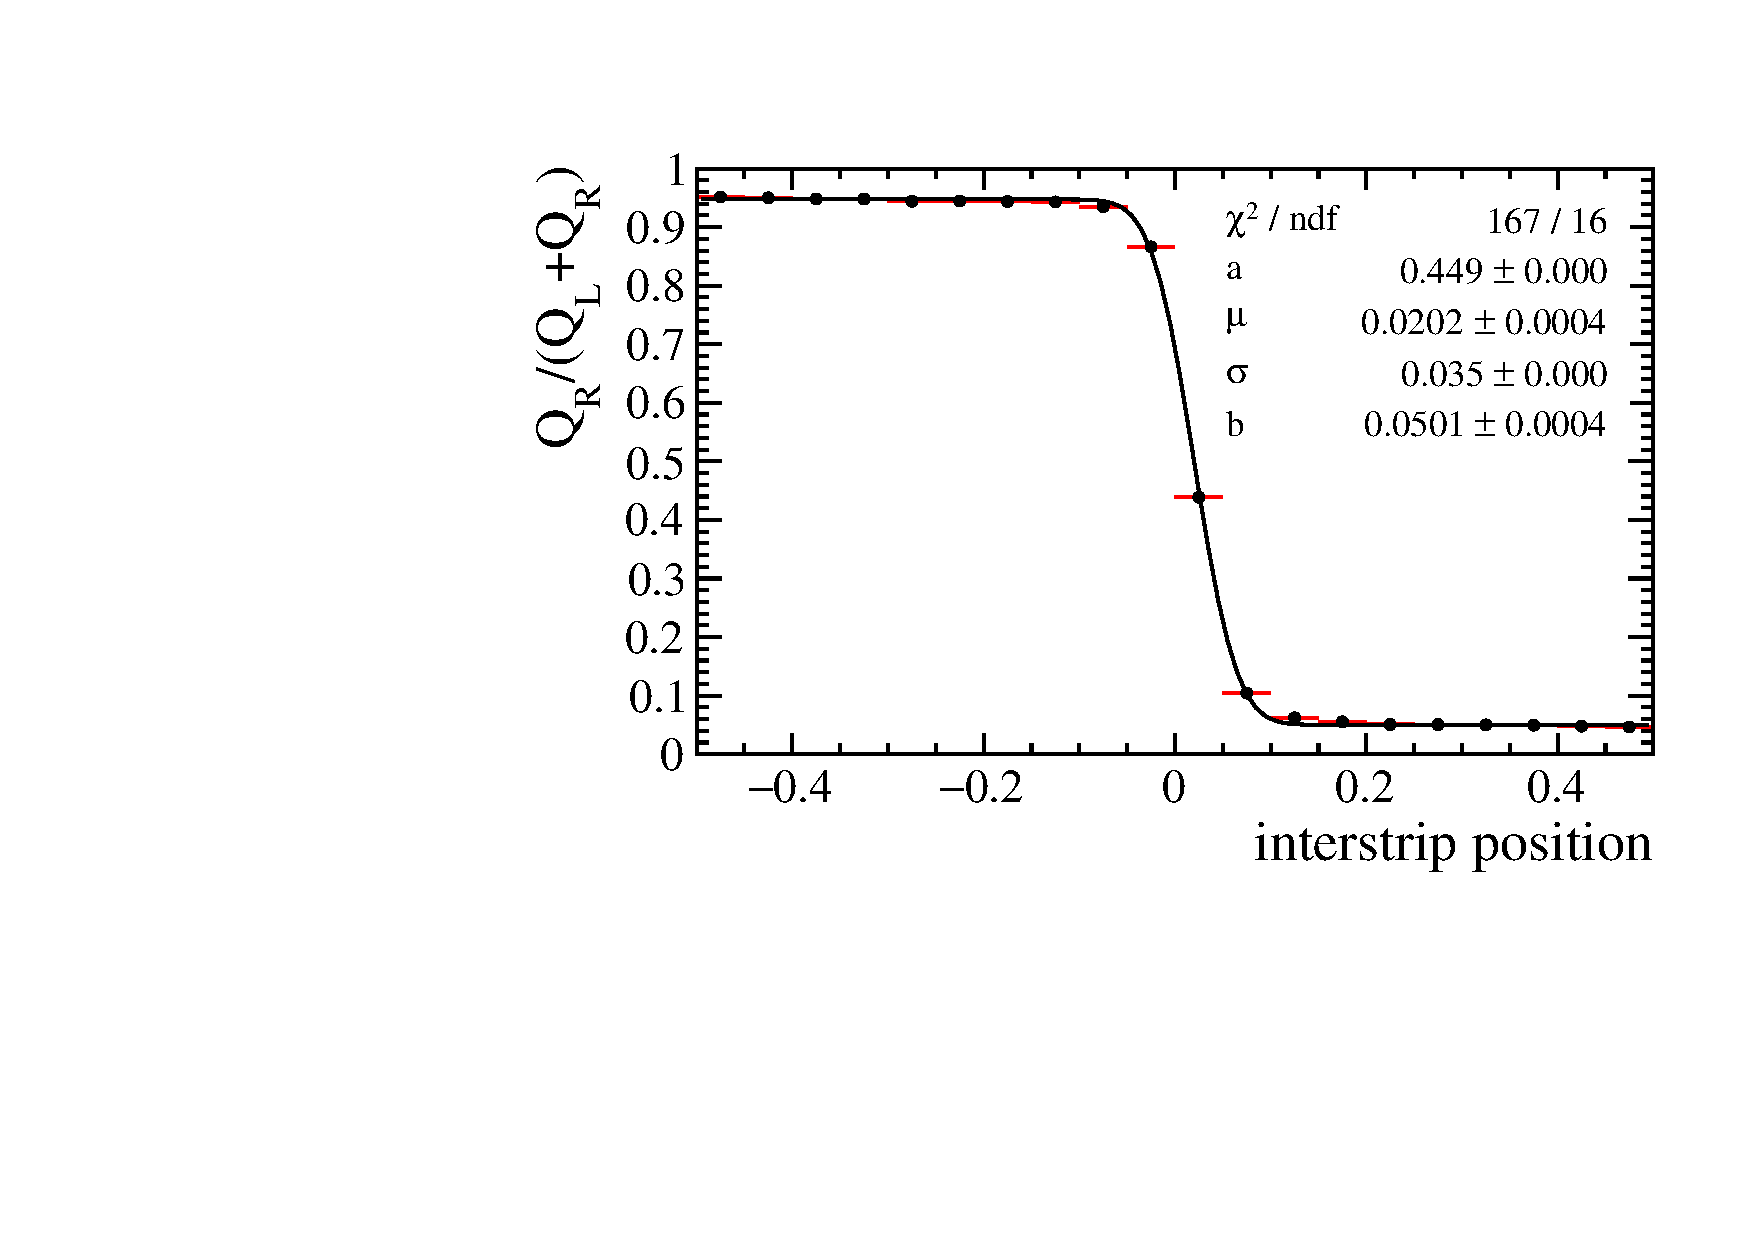
\includegraphics[width=0.4\textwidth]{figs/ChargeSharingvsAngle/cchargeSharing_M3_FanUp_Top_0.pdf}
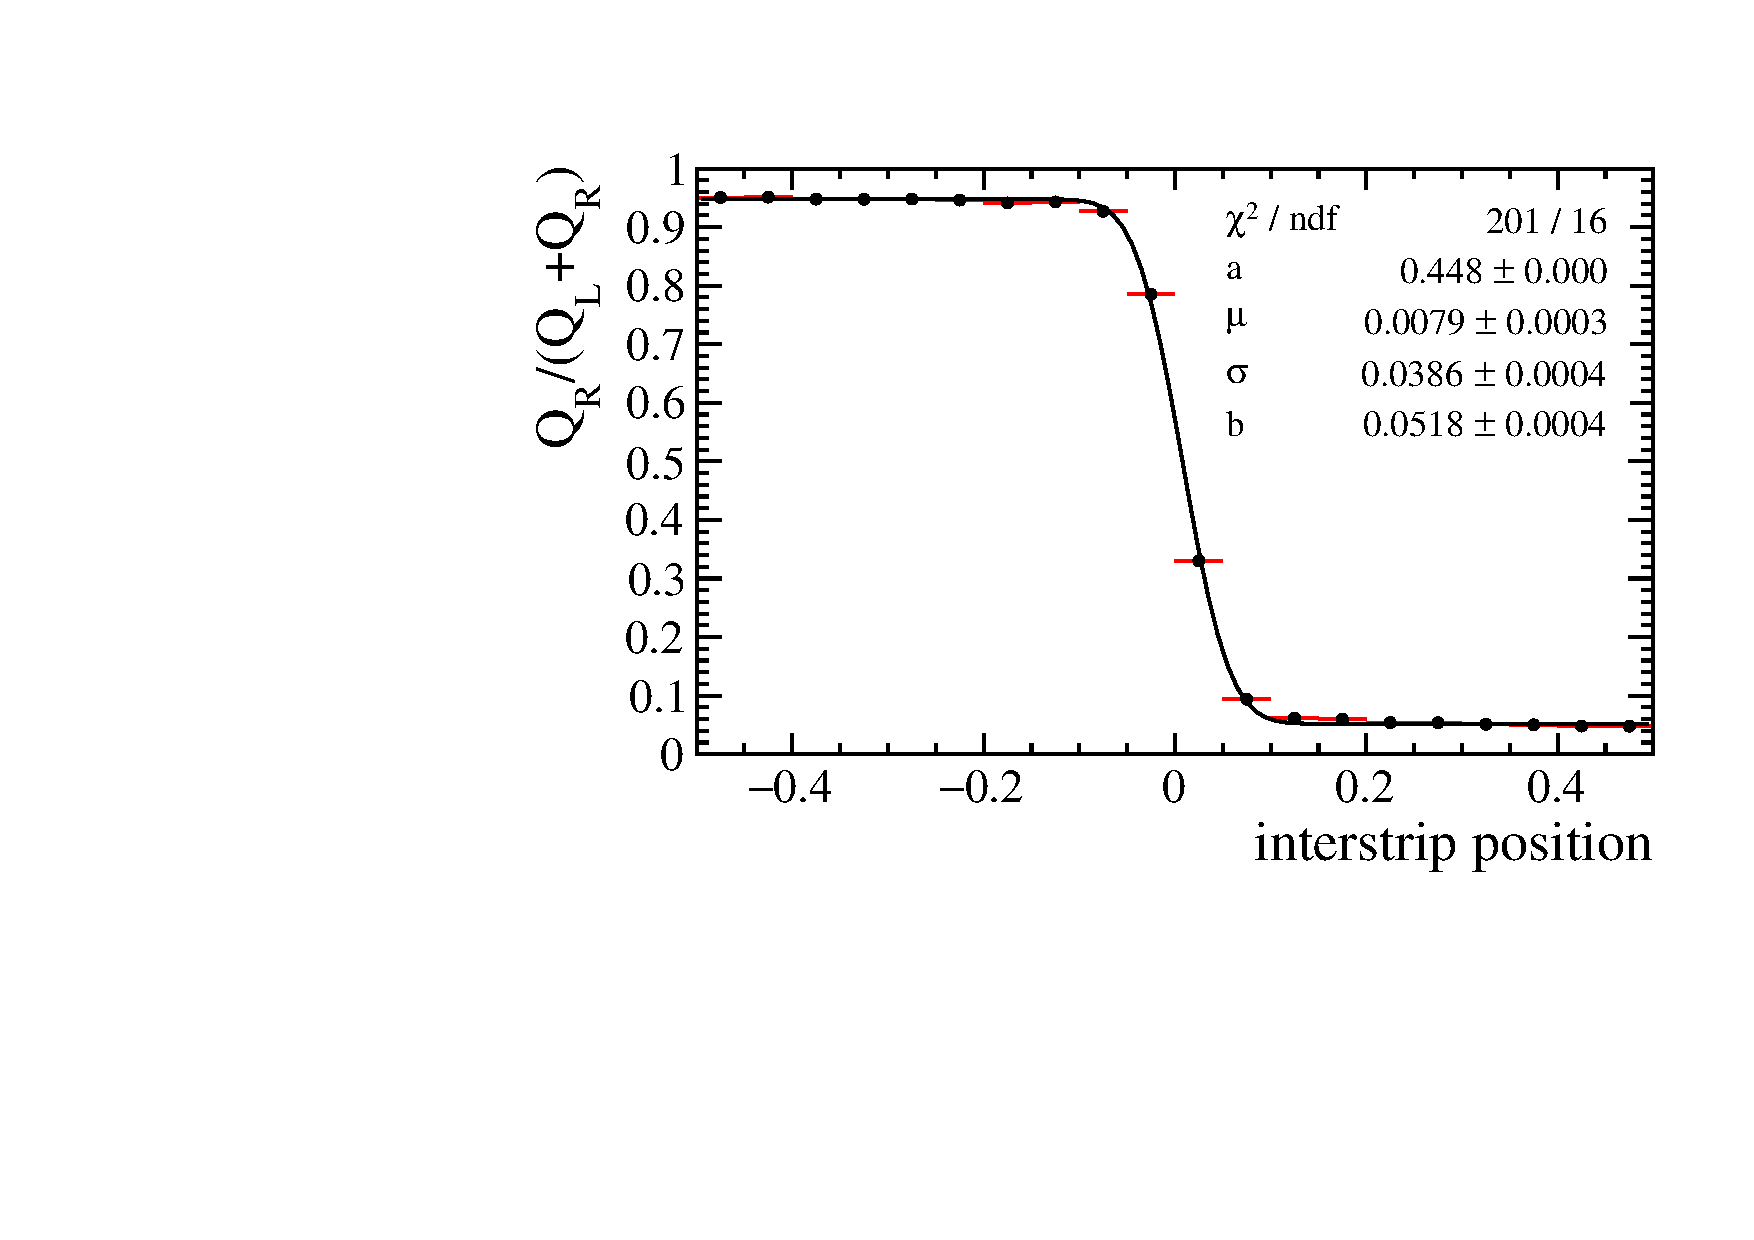
\includegraphics[width=0.4\textwidth]{figs/ChargeSharingvsAngle/cchargeSharing_M3_FanUp_Top_2.pdf}
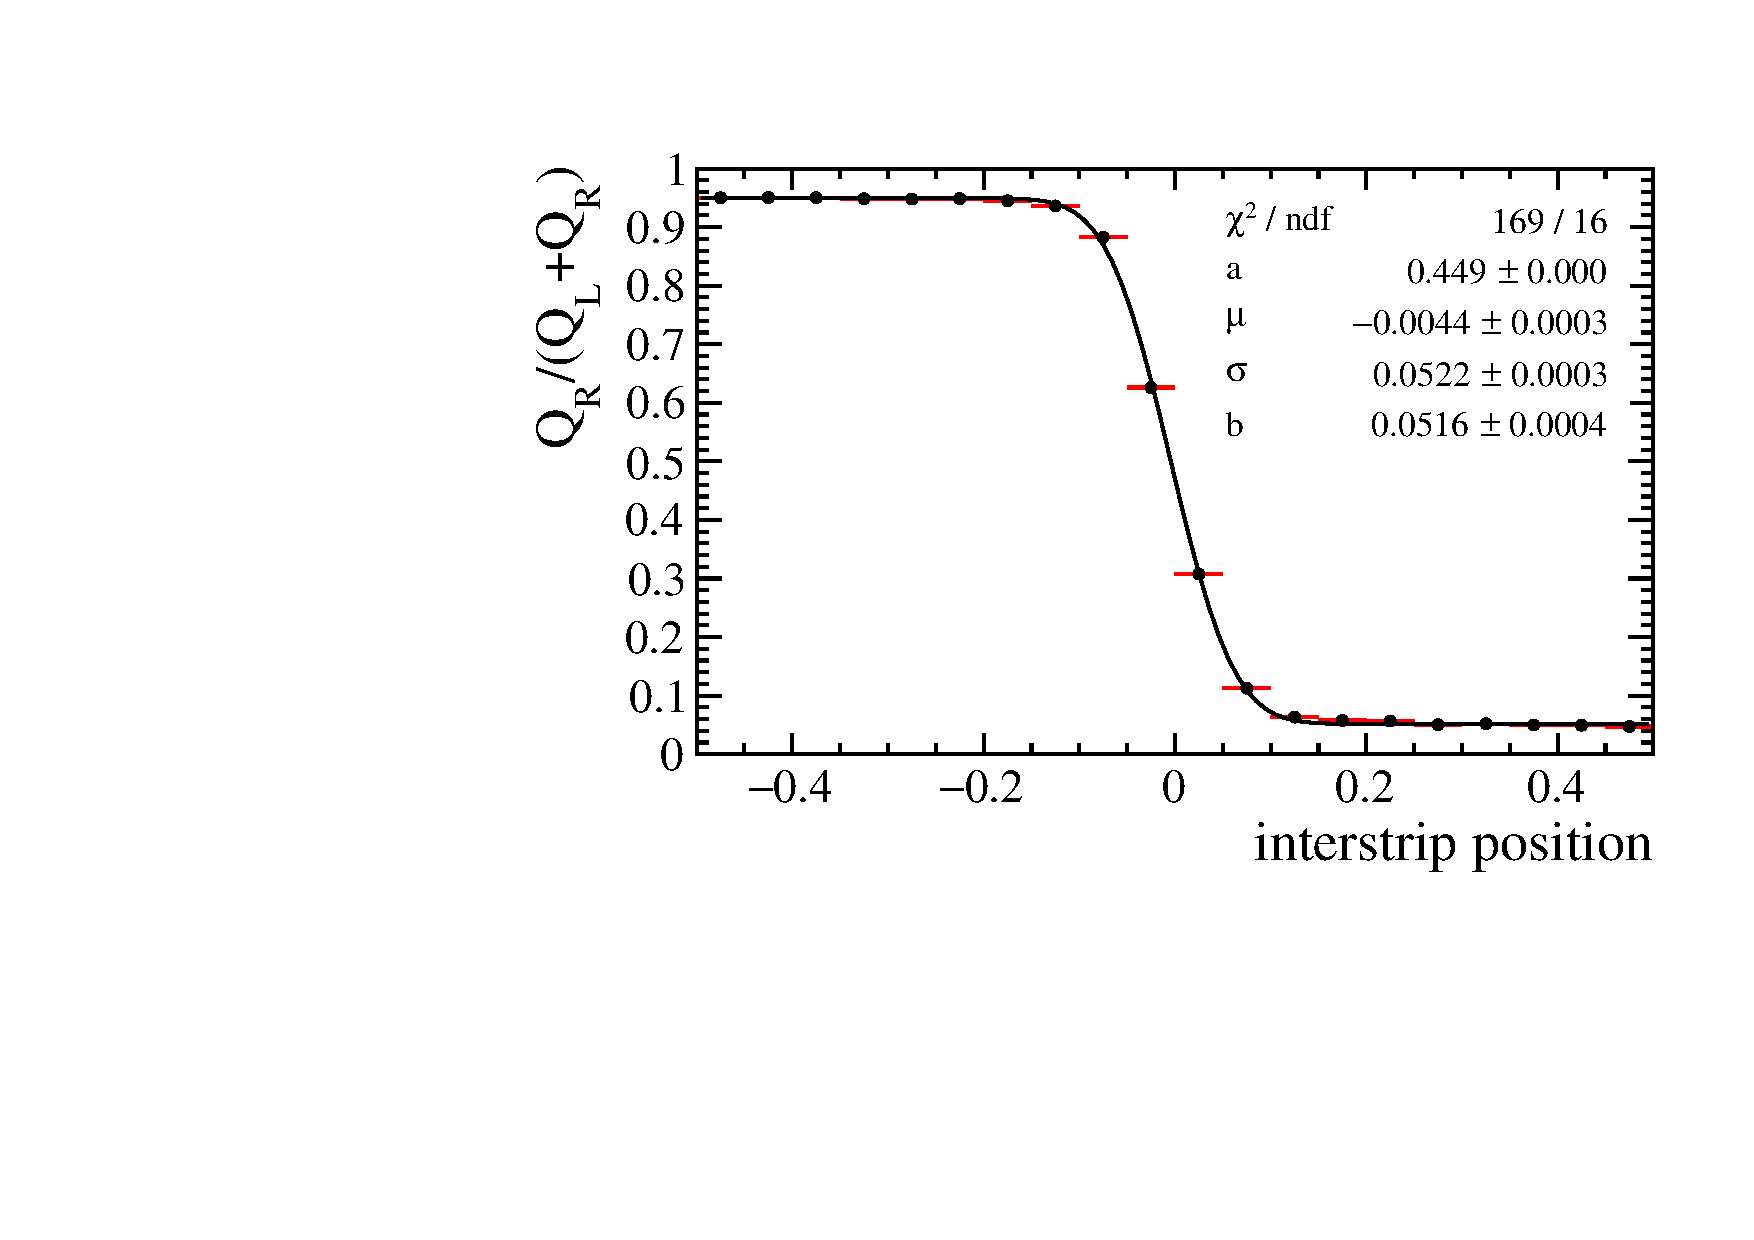
\includegraphics[width=0.4\textwidth]{figs/ChargeSharingvsAngle/cchargeSharing_M3_FanUp_Top_5.pdf}
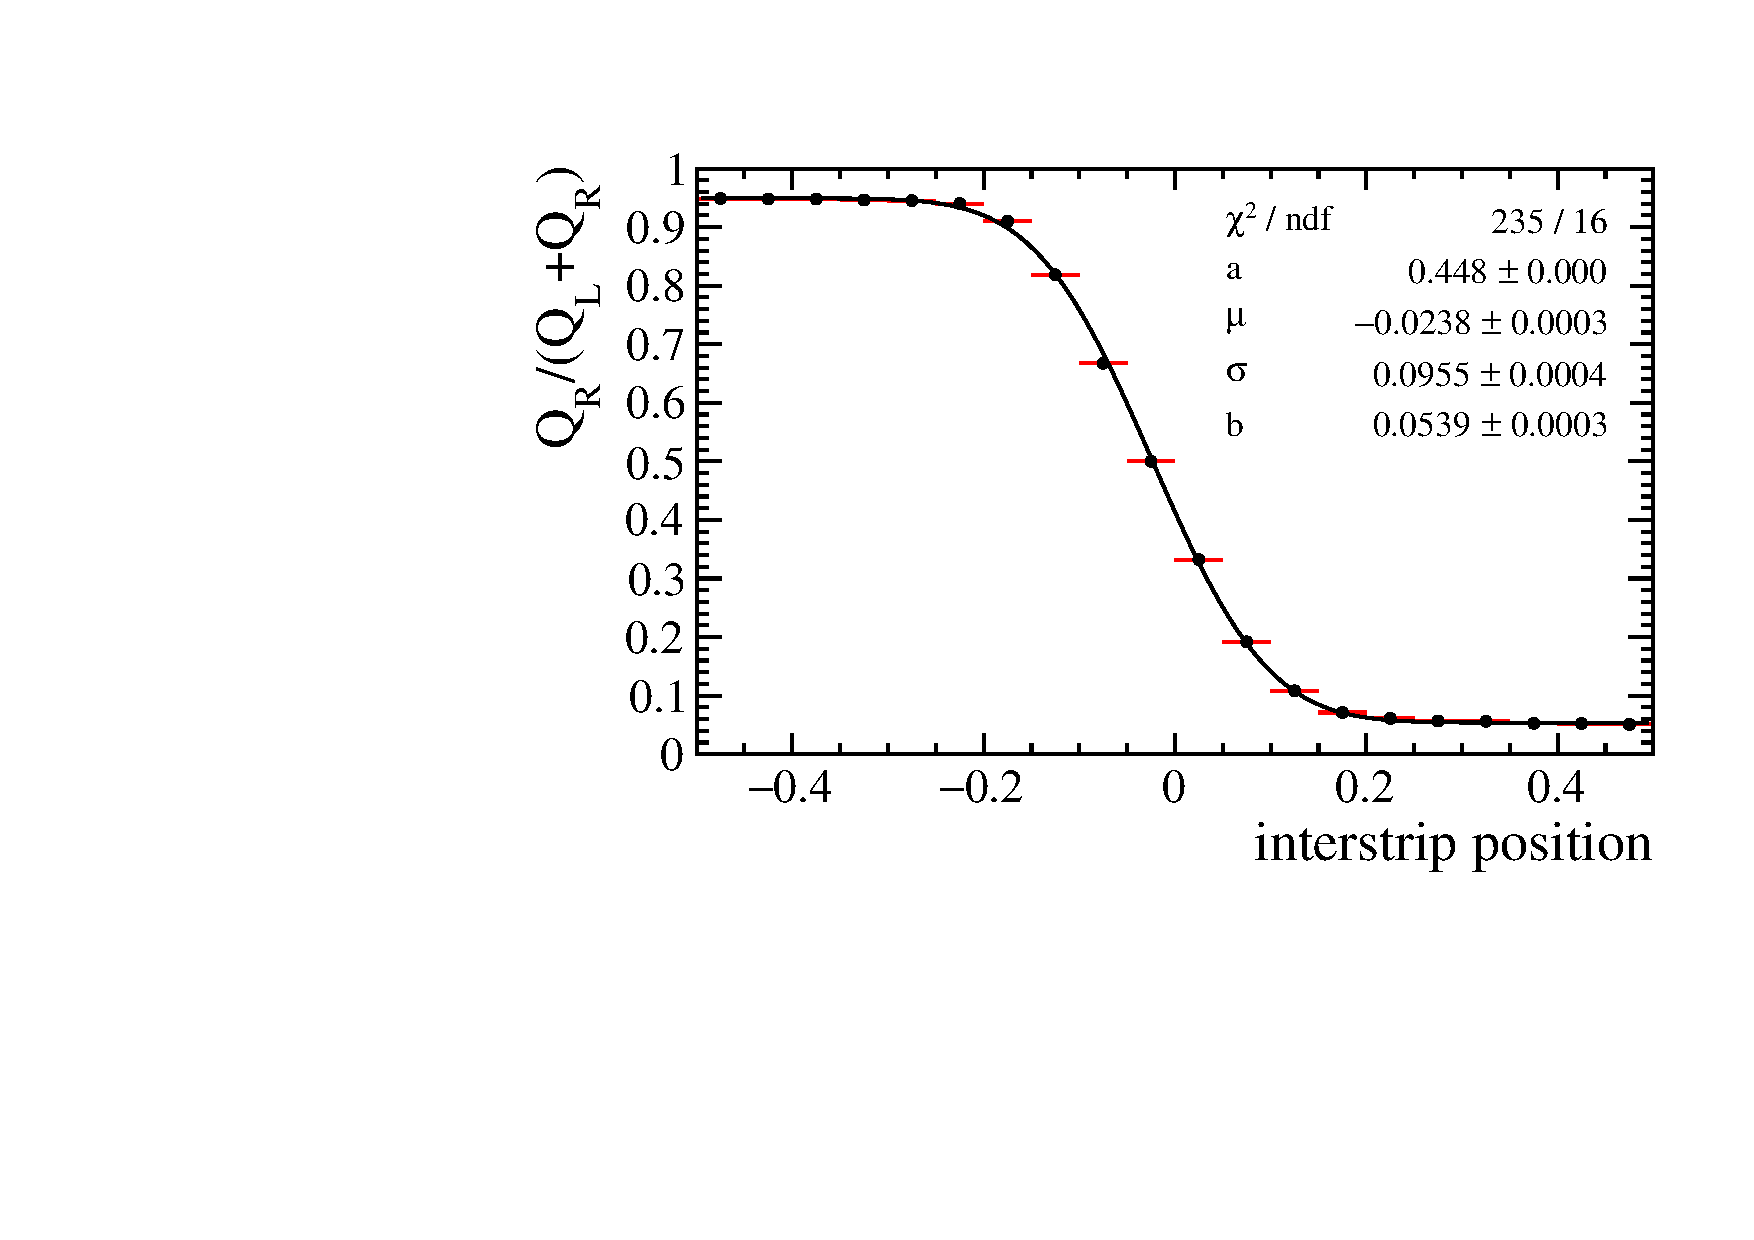
\includegraphics[width=0.4\textwidth]{figs/ChargeSharingvsAngle/cchargeSharing_M3_FanUp_Top_10.pdf}
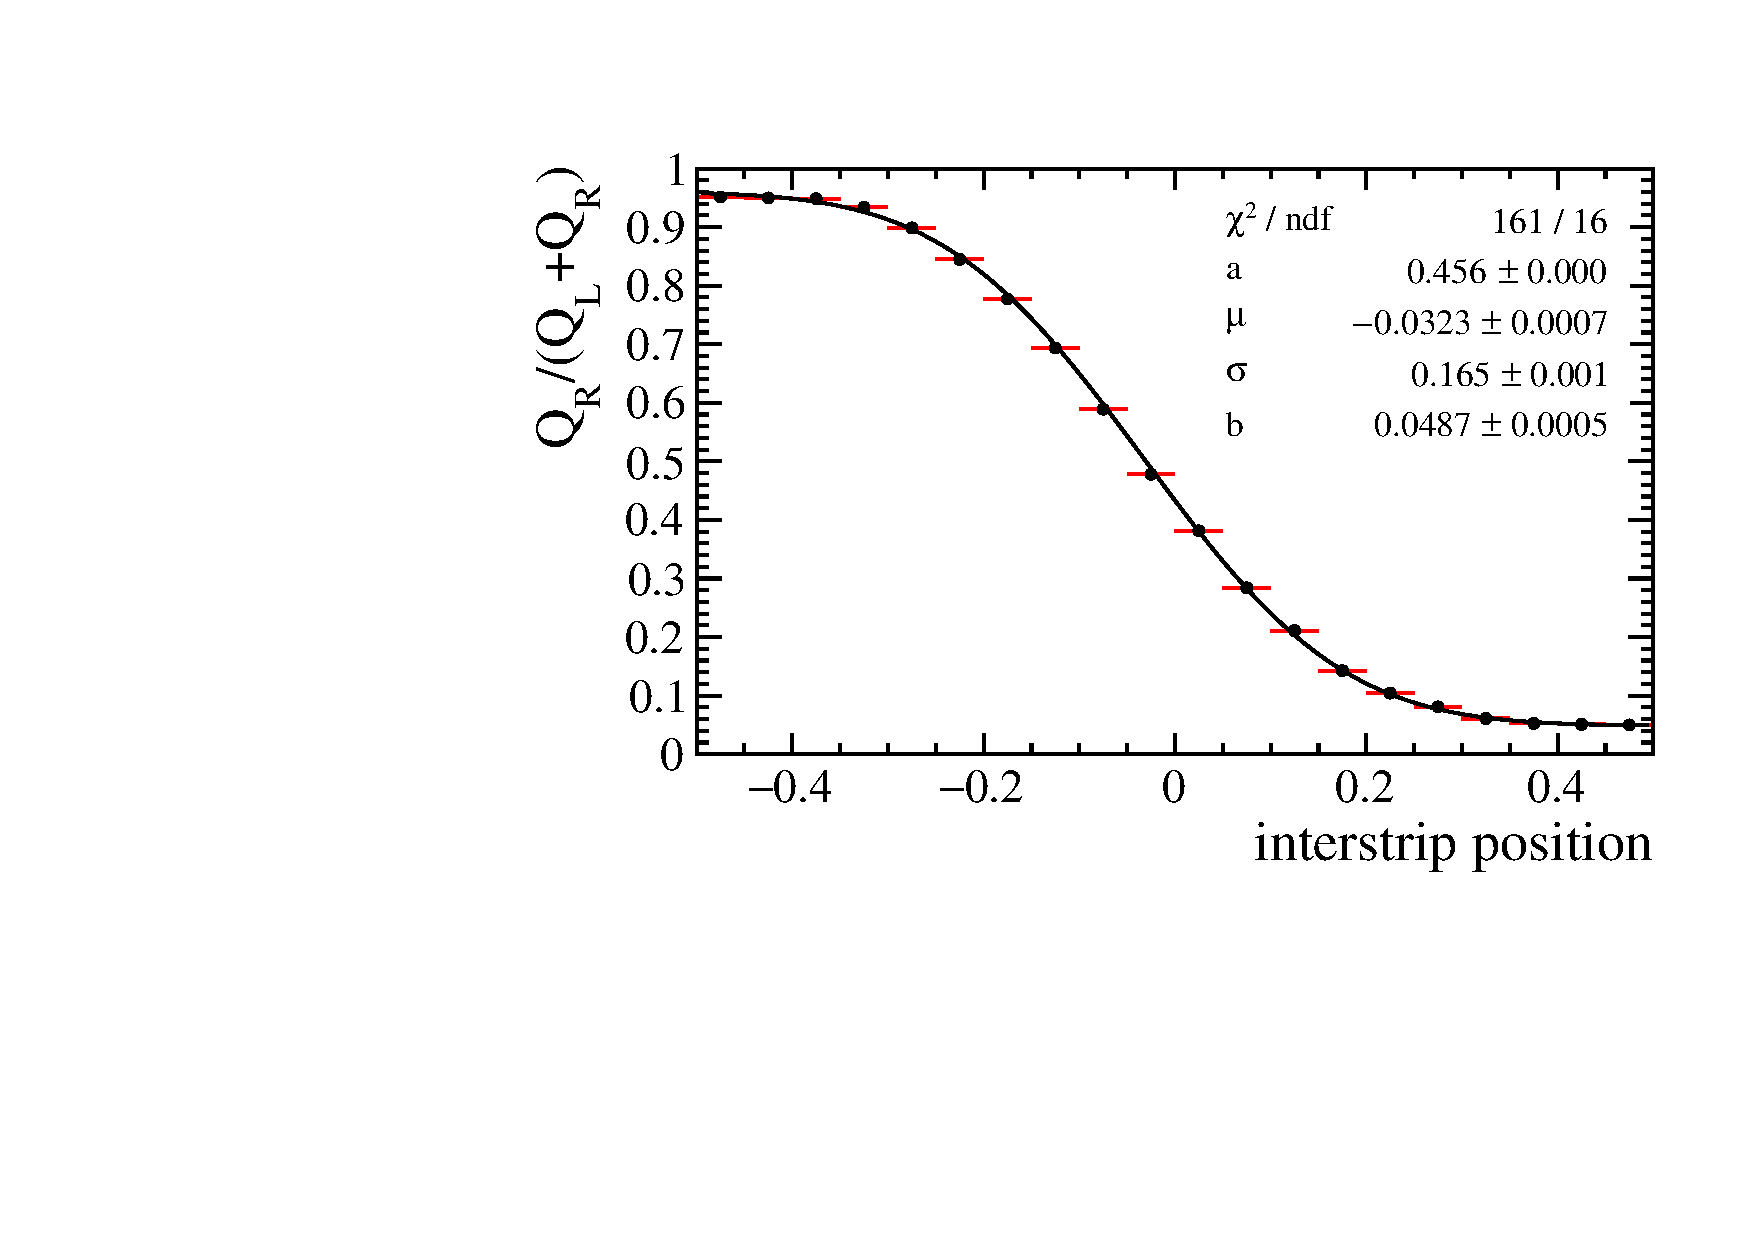
\includegraphics[width=0.4\textwidth]{figs/ChargeSharingvsAngle/cchargeSharing_M3_FanUp_Top_15.pdf}
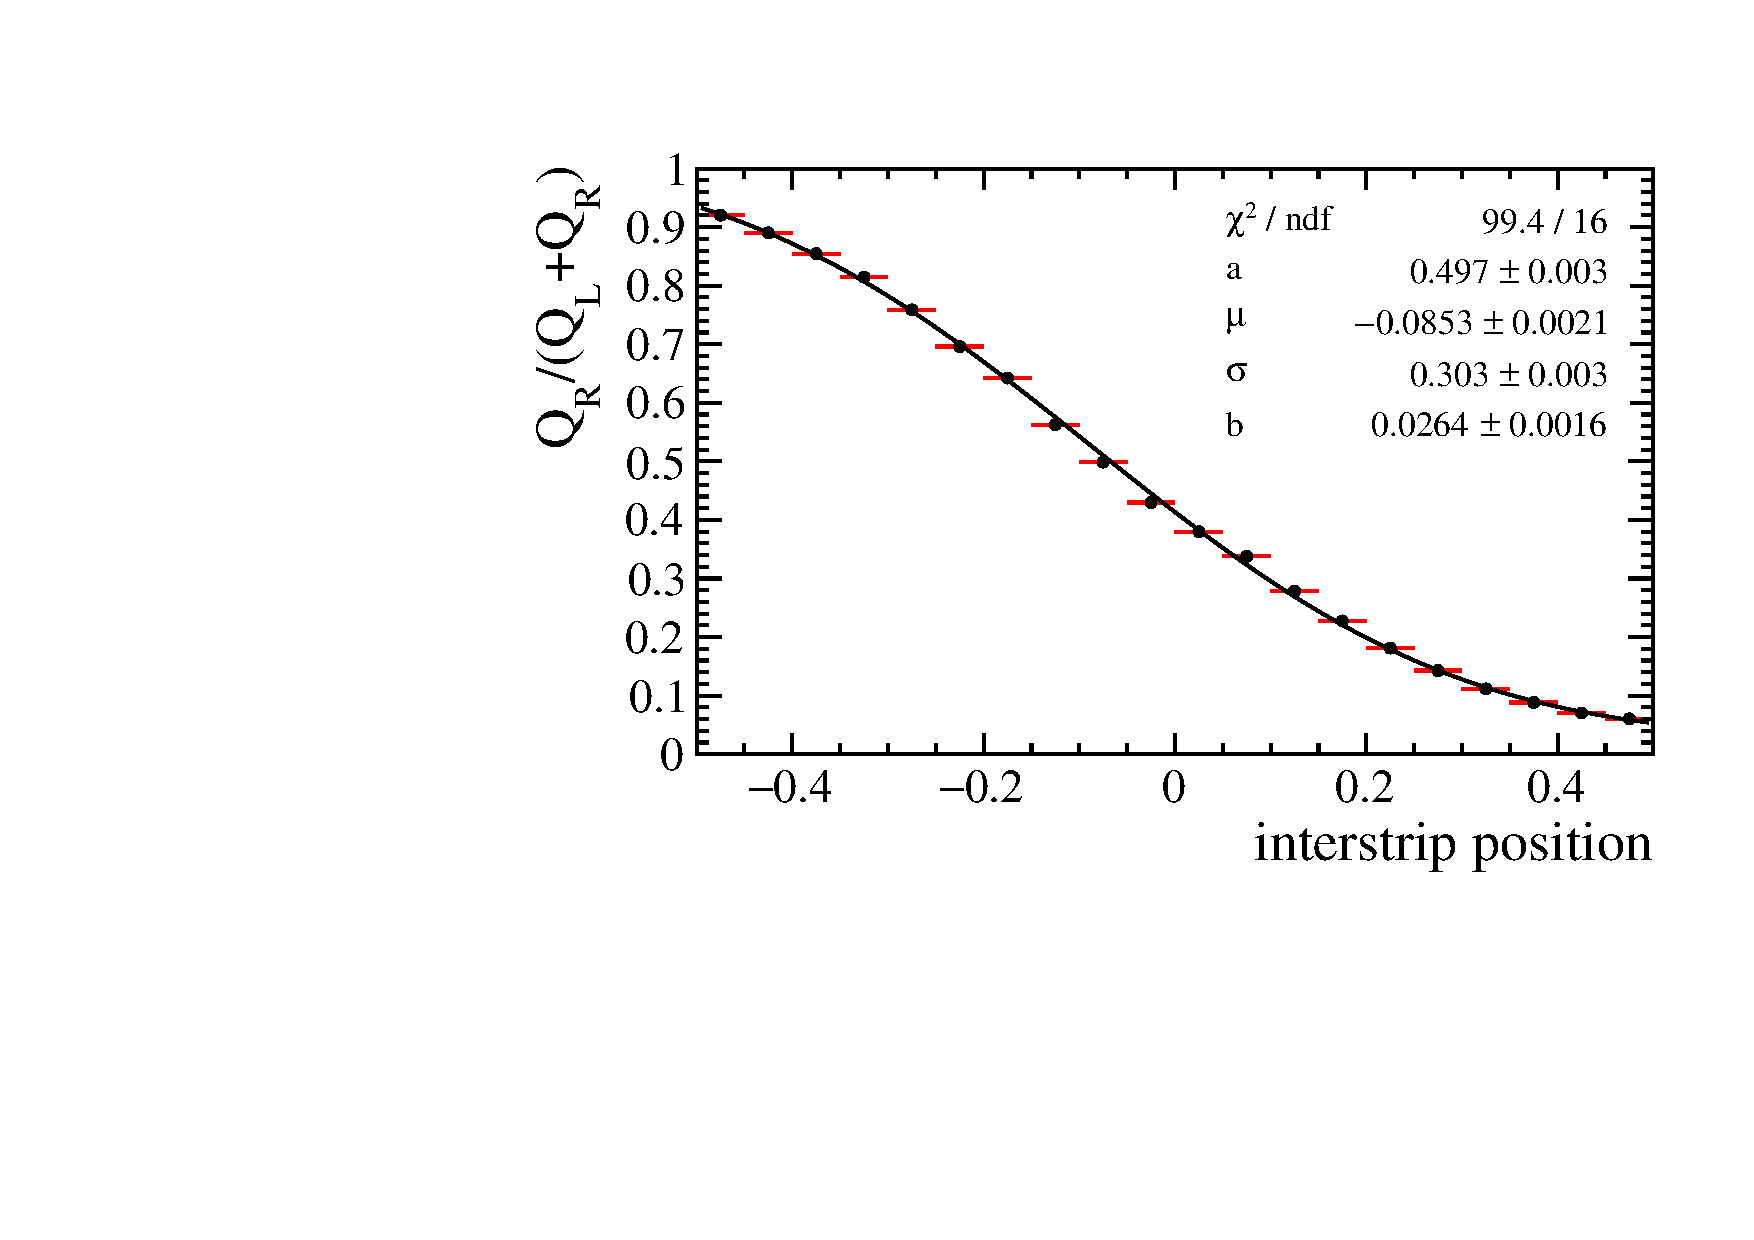
\includegraphics[width=0.4\textwidth]{figs/ChargeSharingvsAngle/cchargeSharing_M3_FanUp_Top_20.pdf}
\caption[Charge sharing as a function of the cluster interstrip position for different rotations around the $y$ axis.]{Charge sharing as a function of the cluster interstrip position for different rotations around the $y$ axis, as obtained for the M3 fan-up sensor with top biasing. The rotations around the $y$ axis are $-10^\circ$ (first row left), $-5^\circ$ (first row right), $-2^\circ$ (second row left), $0^\circ$ (second row right), $2^\circ$ (third row left), $5^\circ$ (third row right), $10^\circ$ (fourth row left), $15^\circ$ (fourth row right), and $20^\circ$ (fifth row).}
\label{fig:ChargeSharingvsAngle}
\end{figure}

\begin{figure}[]
\centering
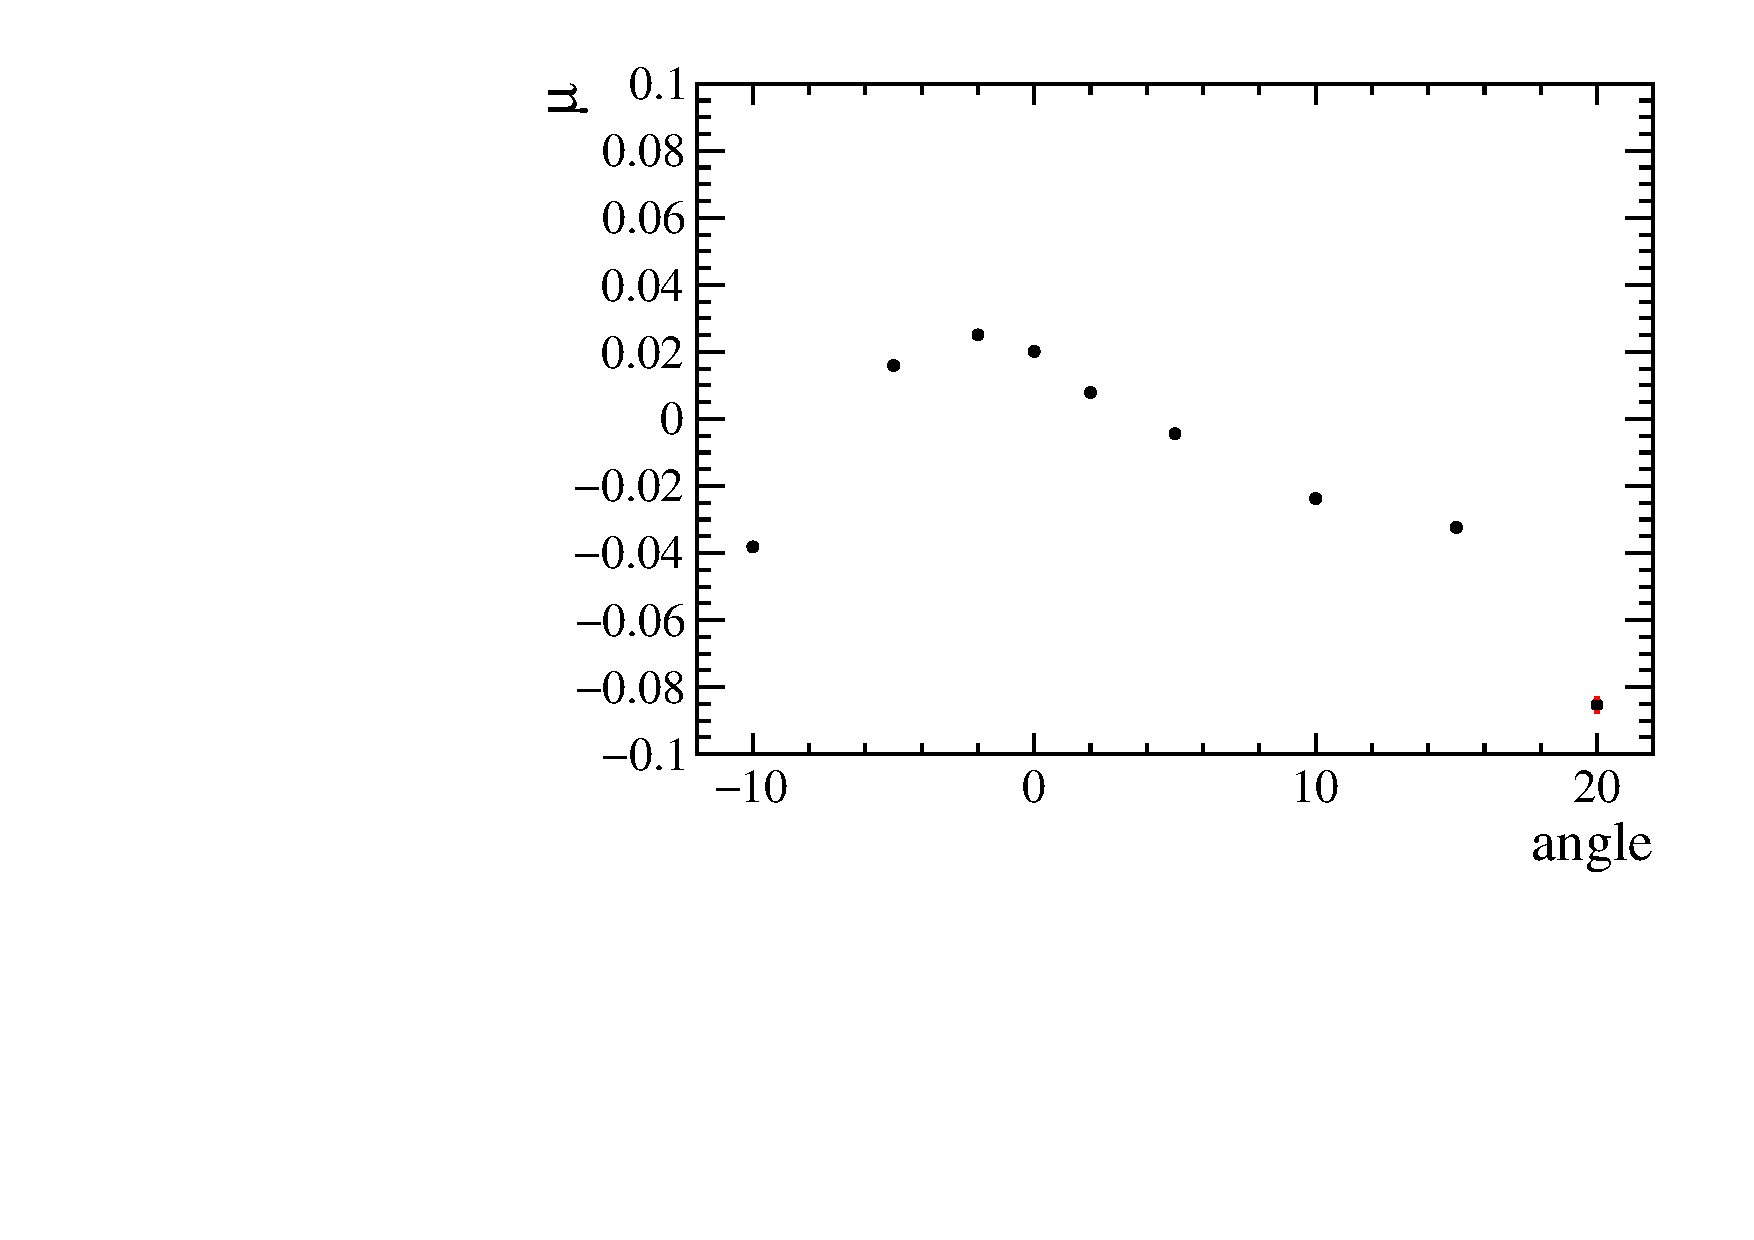
\includegraphics[width=0.45\textwidth]{figs/ChargeSharingvsAngle/cmuvsAngle_M3_FanUp_Top.pdf}
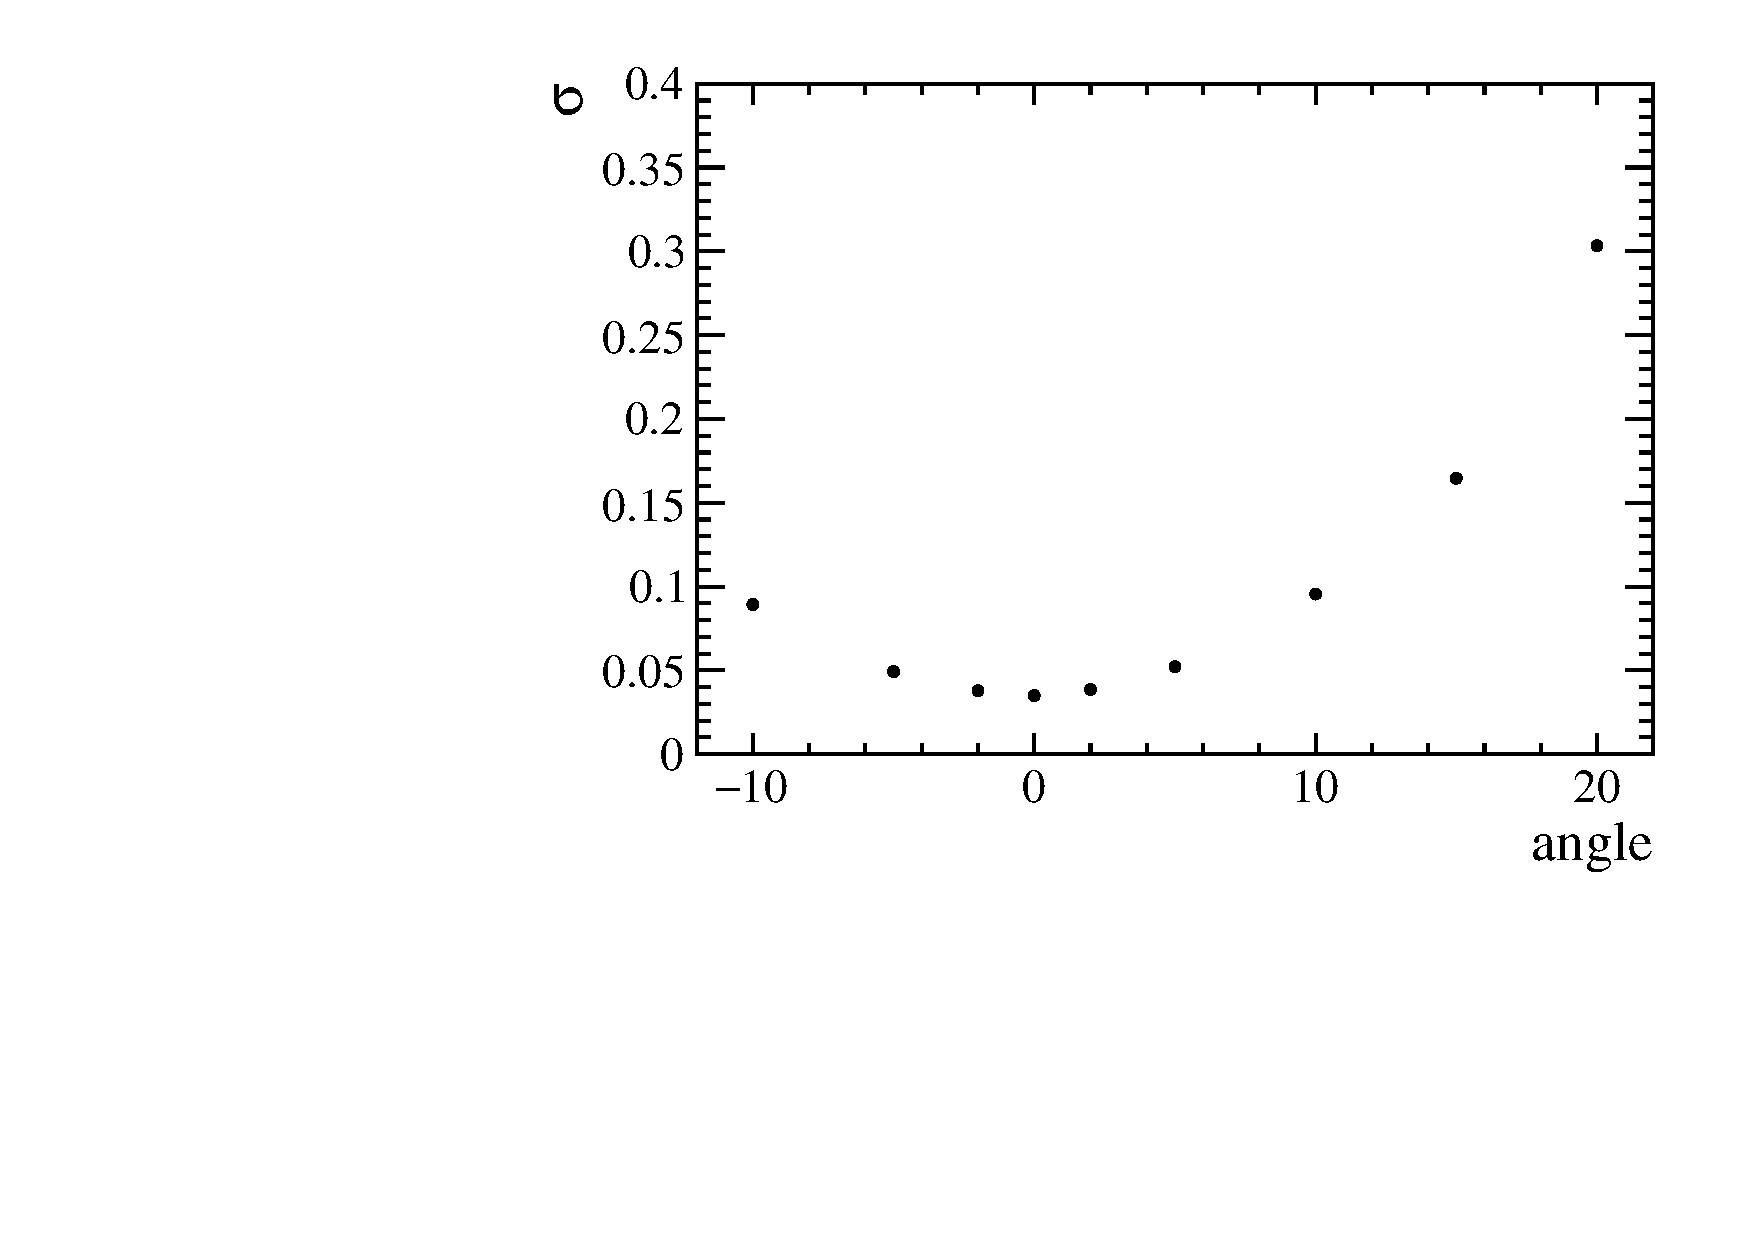
\includegraphics[width=0.45\textwidth]{figs/ChargeSharingvsAngle/csigmavsAngle_M3_FanUp_Top.pdf}
\caption[Dependence of the parameters $\mu$ and $\sigma$ on the rotation around the $y$ axis.]{Dependence of the parameters $\mu$ (left) and $\sigma$ (right) on the rotation around the $y$ axis, as obtained for the M3 fan-up sensor with top biasing.}
\label{fig:ChargeSharingvsAngle2}
\end{figure}

\subsection{Rotations around the $y$ axis}

A misalignment of the DUT around the $y$ axis would manifest itself as...

The MPV of the Landau distribution as a function of the rotation around the $y$ axis is shown in Fig. \ref{fig:SNRvsAngle} for the M1 fan-in (left) and M1 fan-up (right) sensors.
The MPV is expected to be symmetric with respect to the angle for which the beam hit the DUT at normal incidence.
As the rotation around the $y$ axis increases, the particles traverse more material and consequently release more energy, which leads to a larger deposited charge and hence a larger MPV. The increase in the material is proportional to $\cos\theta^{-1}$, where $\theta$ is the angle with respect to the perpendicular to the DUT plane.
The dependence between MPV and rotation around the $y$ axis is assumed to be
\begin{displaymath}
\frac{a}{\cos(\theta-\alpha)},
\end{displaymath}
where $\alpha$ is the nominal zero angle and $a$ is the corresponding MPV value. 
The fit results for the mini sensors are summarised in Table \ref{tab:RotationY} and are all compatible with zero.

\begin{figure}[]
\centering
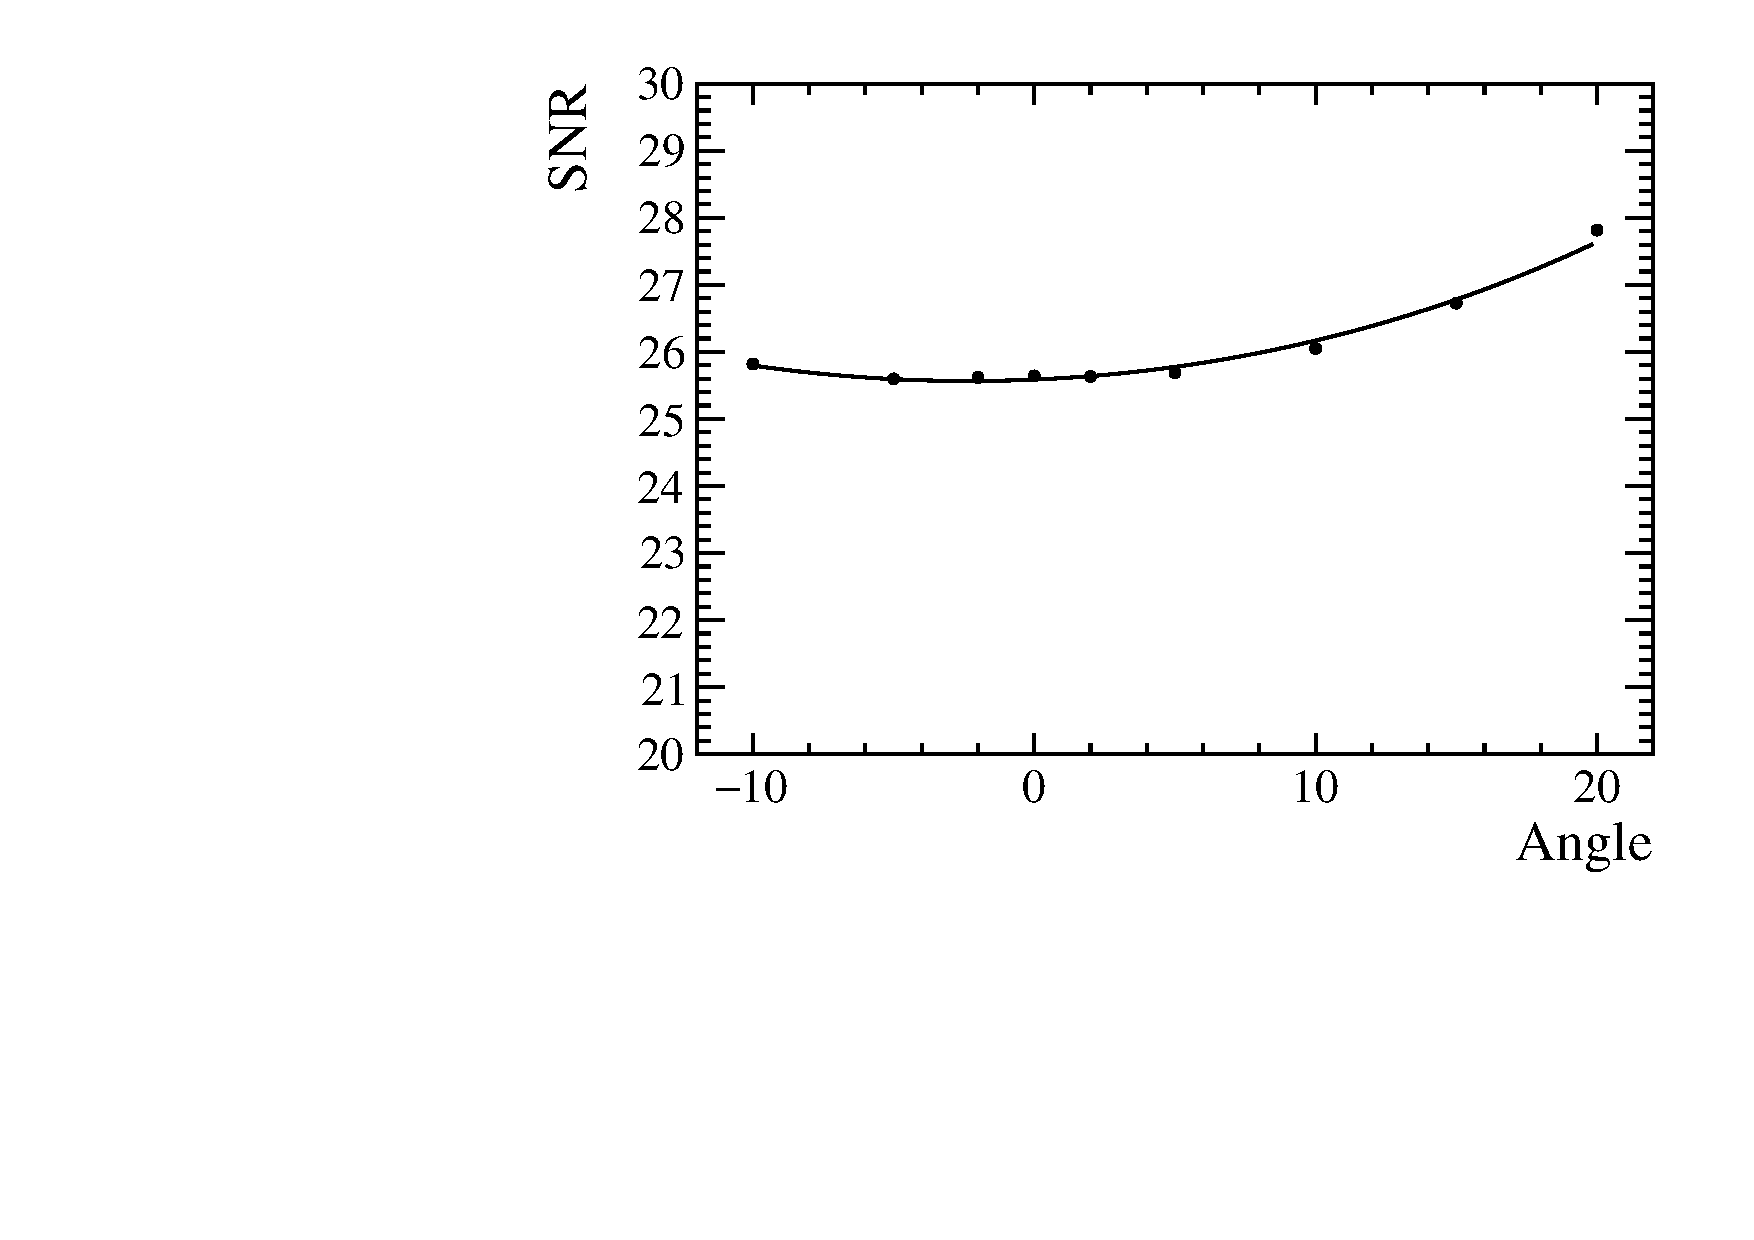
\includegraphics[width=0.45\textwidth]{figs/SNRvsAngle/cSNRvsAngle_M1_FanIn_Top.pdf}
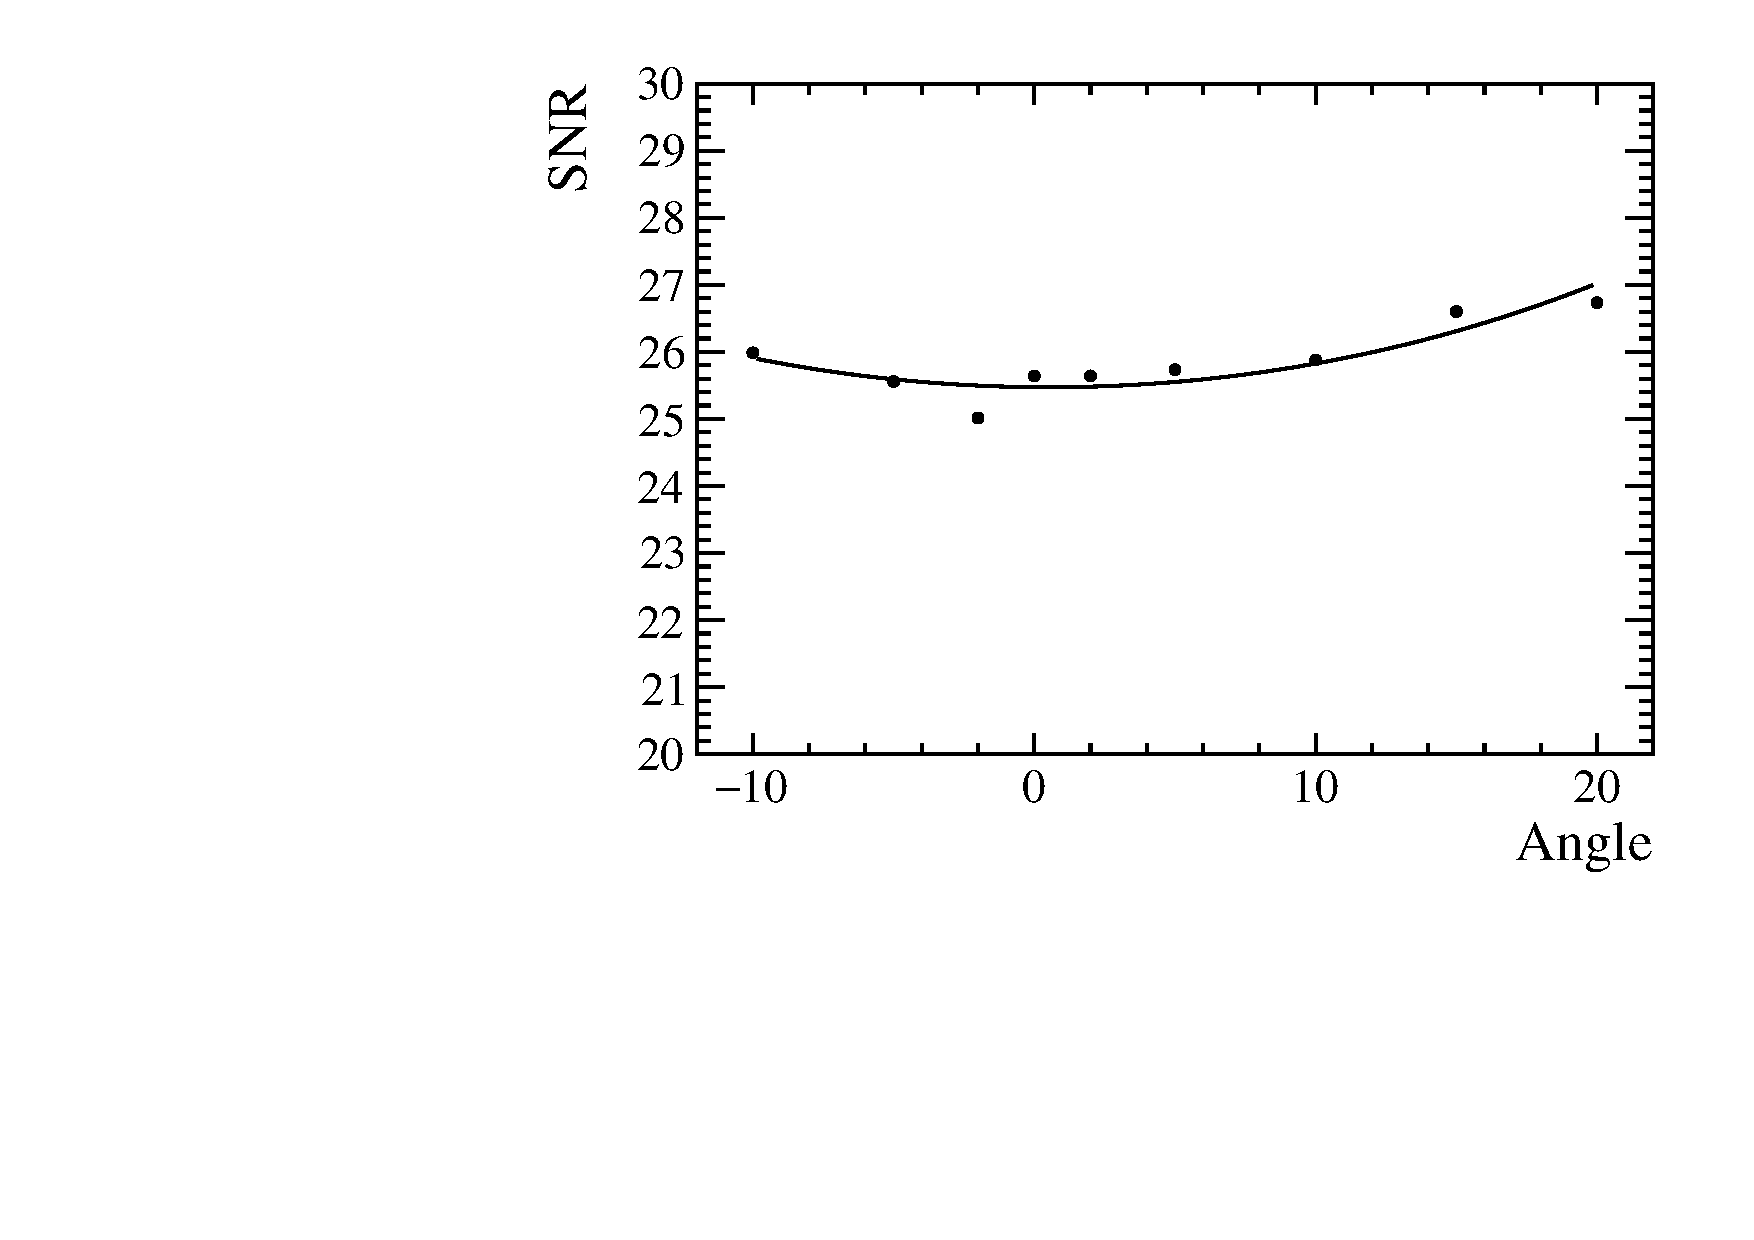
\includegraphics[width=0.45\textwidth]{figs/SNRvsAngle/cSNRvsAngle_M1_FanUp_Back.pdf}
\caption[SNR as a function of the rotation around the $y$ axis.]{SNR as a function of the rotation around the $y$ axis for the M1 fan-in with top biasing (left) and fan-up with back biasing (right) sensors.}
\label{fig:SNRvsAngle}
\end{figure}

A similar cross checks consists in studying the dependence of the fraction of one-strip and two-strip clusters on the rotation around the $y$ axis. Similarly to what discussed above, these distributions are expected to be symmetric with respect to the nominal zero angle, which can be determined by performing a fit with a second-order polynomial function. This is a very simple hypothesis and does not reproduce the real shape of the distribution for rotations larger than few degrees, but is sufficient to determine the symmetry point.

\begin{figure}[]
\centering
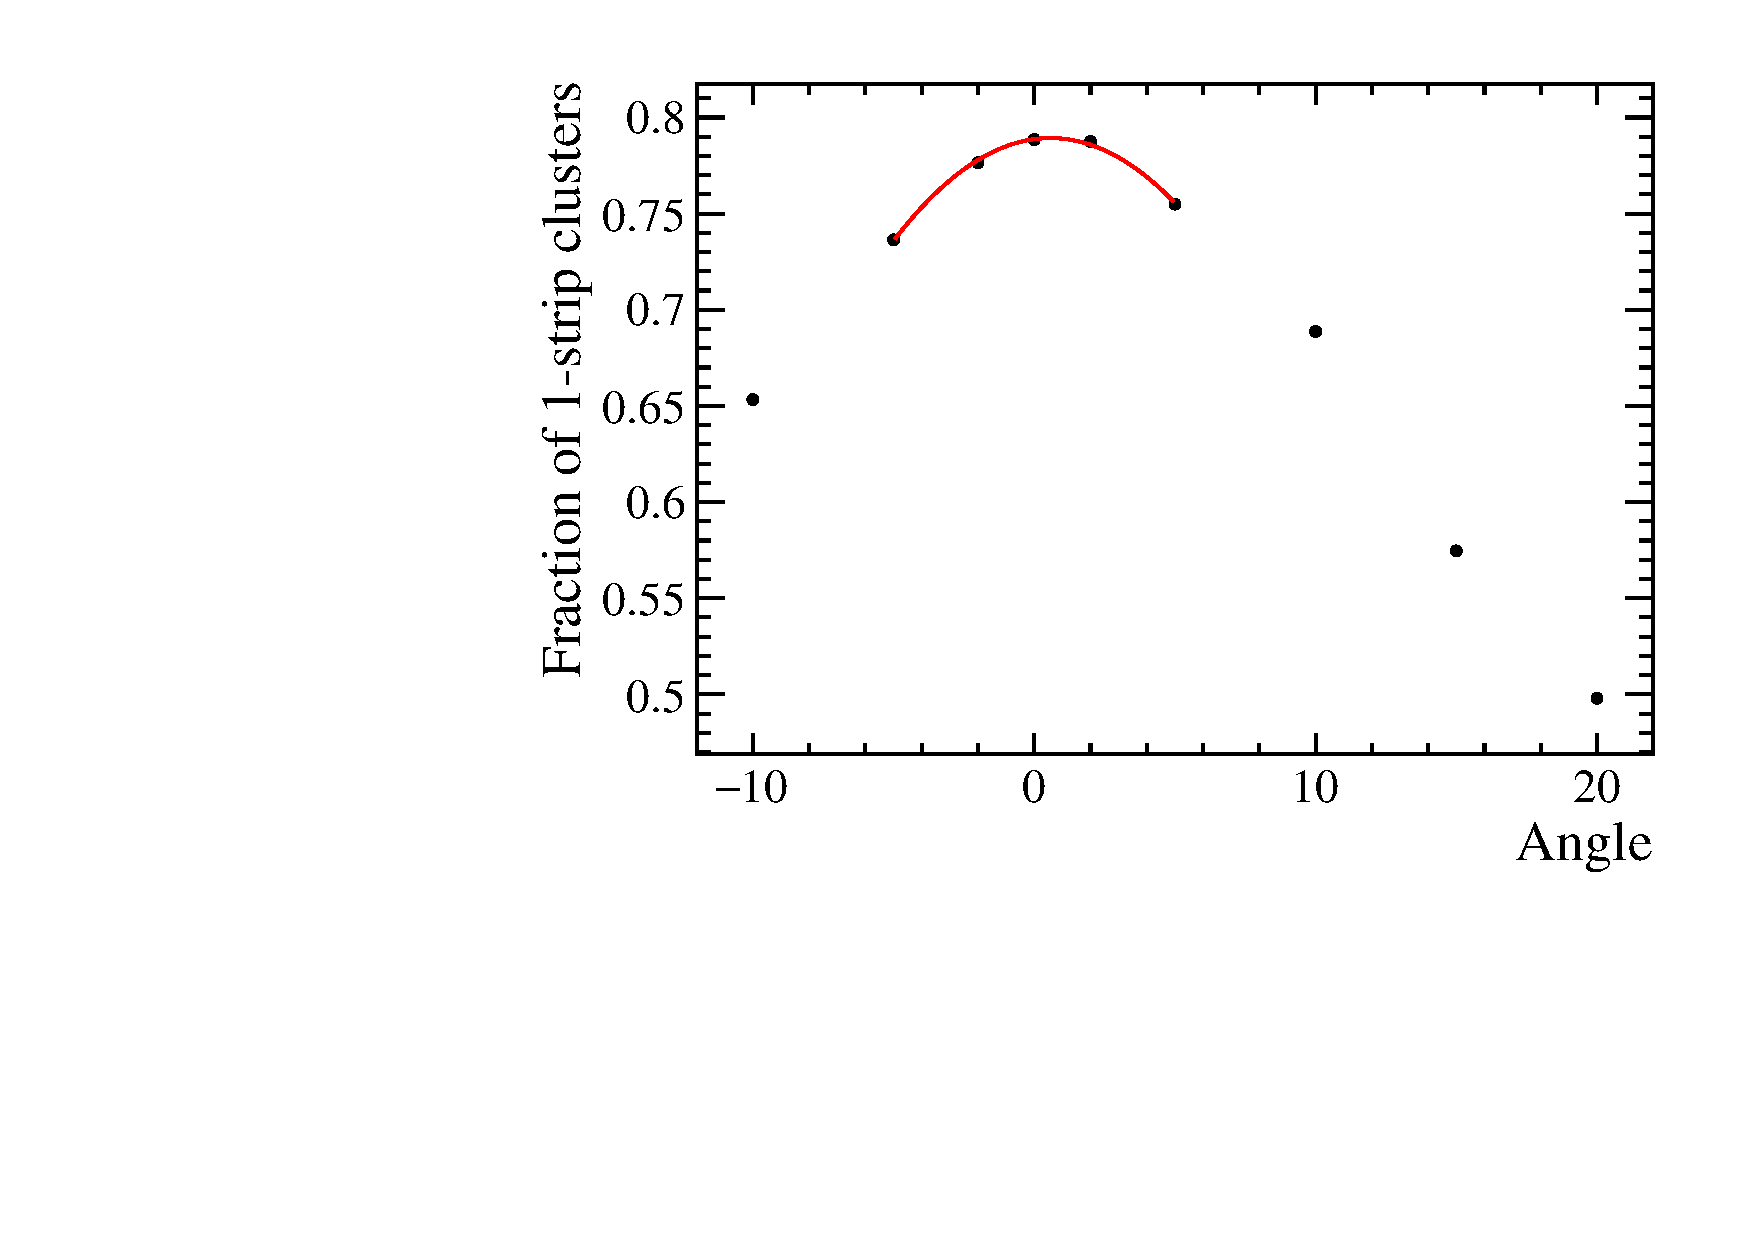
\includegraphics[width=0.45\textwidth]{figs/SNRvsAngle/cf1StripClustervsAngle_M4_FanIn_Top.pdf}
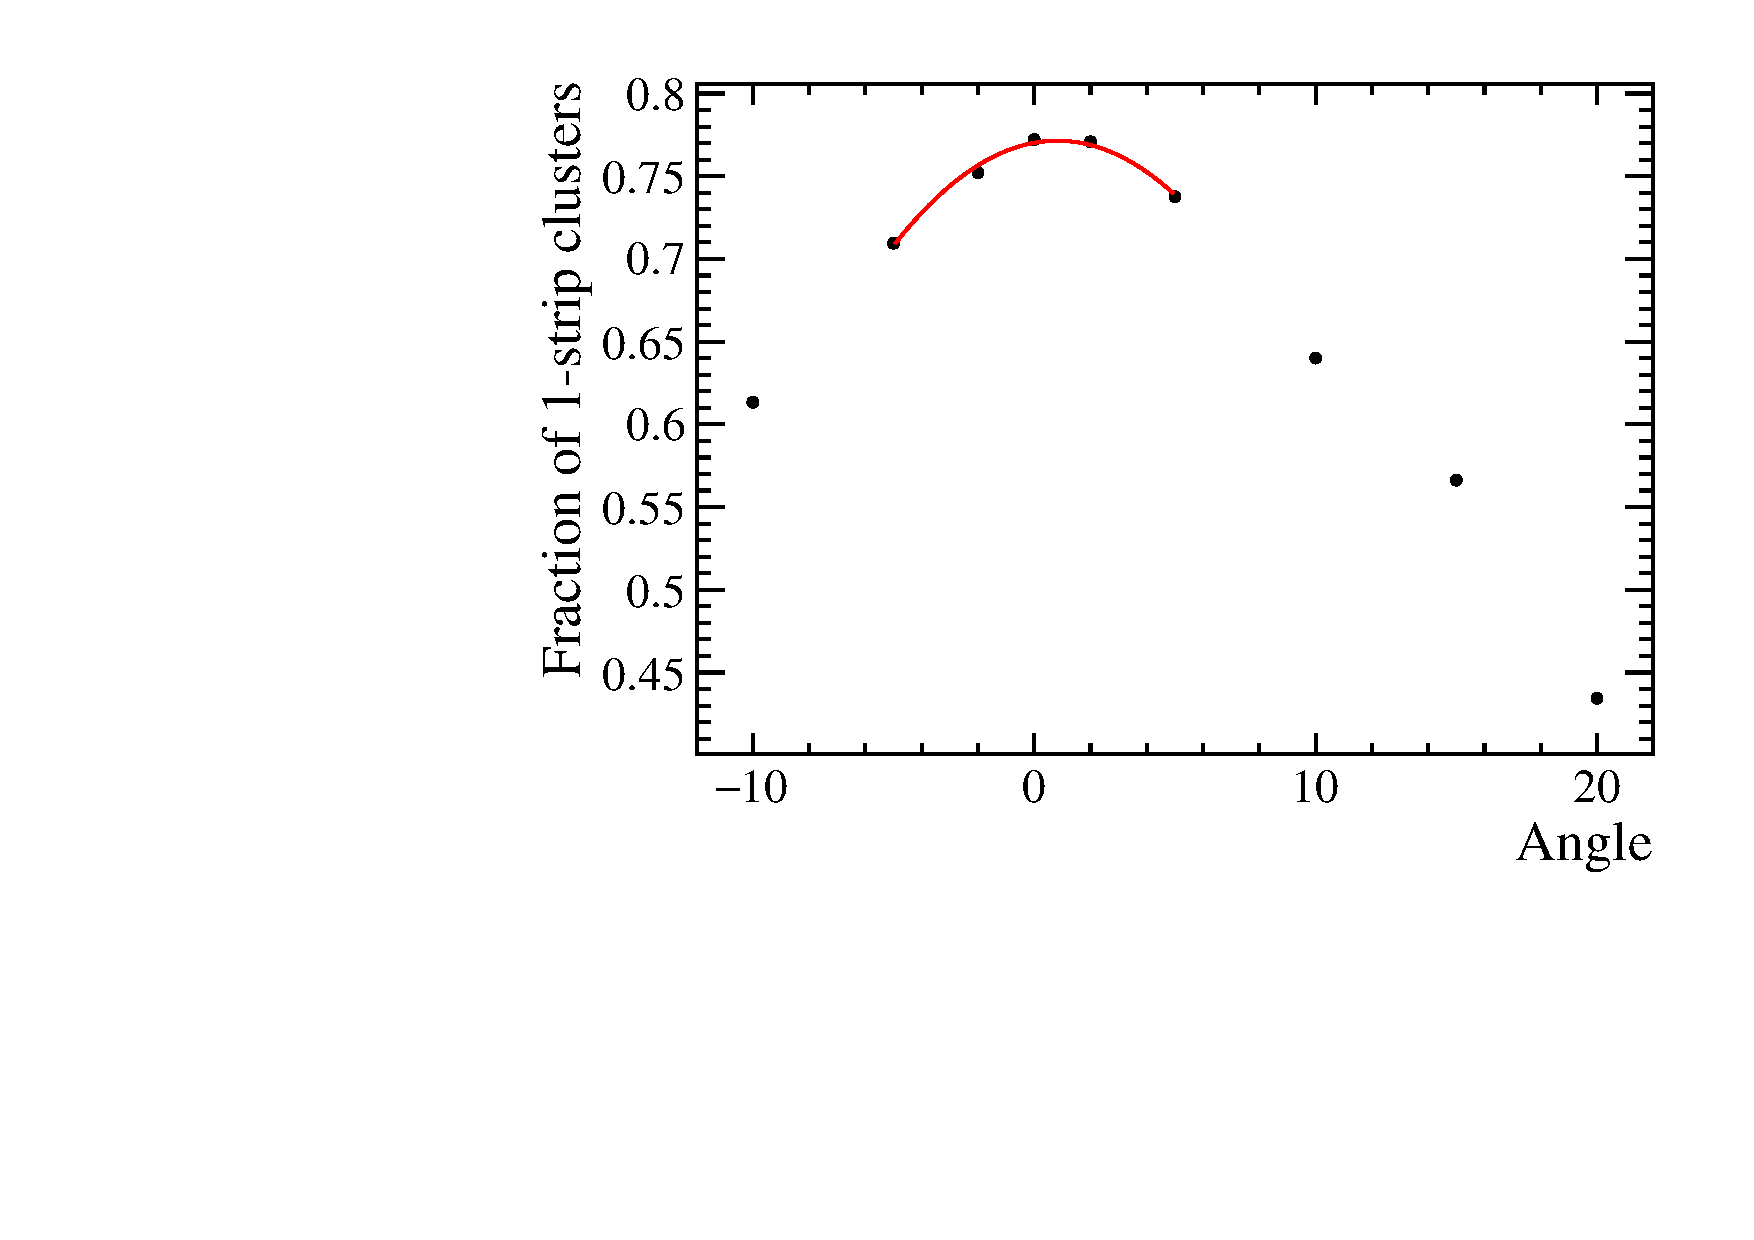
\includegraphics[width=0.45\textwidth]{figs/SNRvsAngle/cf1StripClustervsAngle_M4_FanUp_Top.pdf}
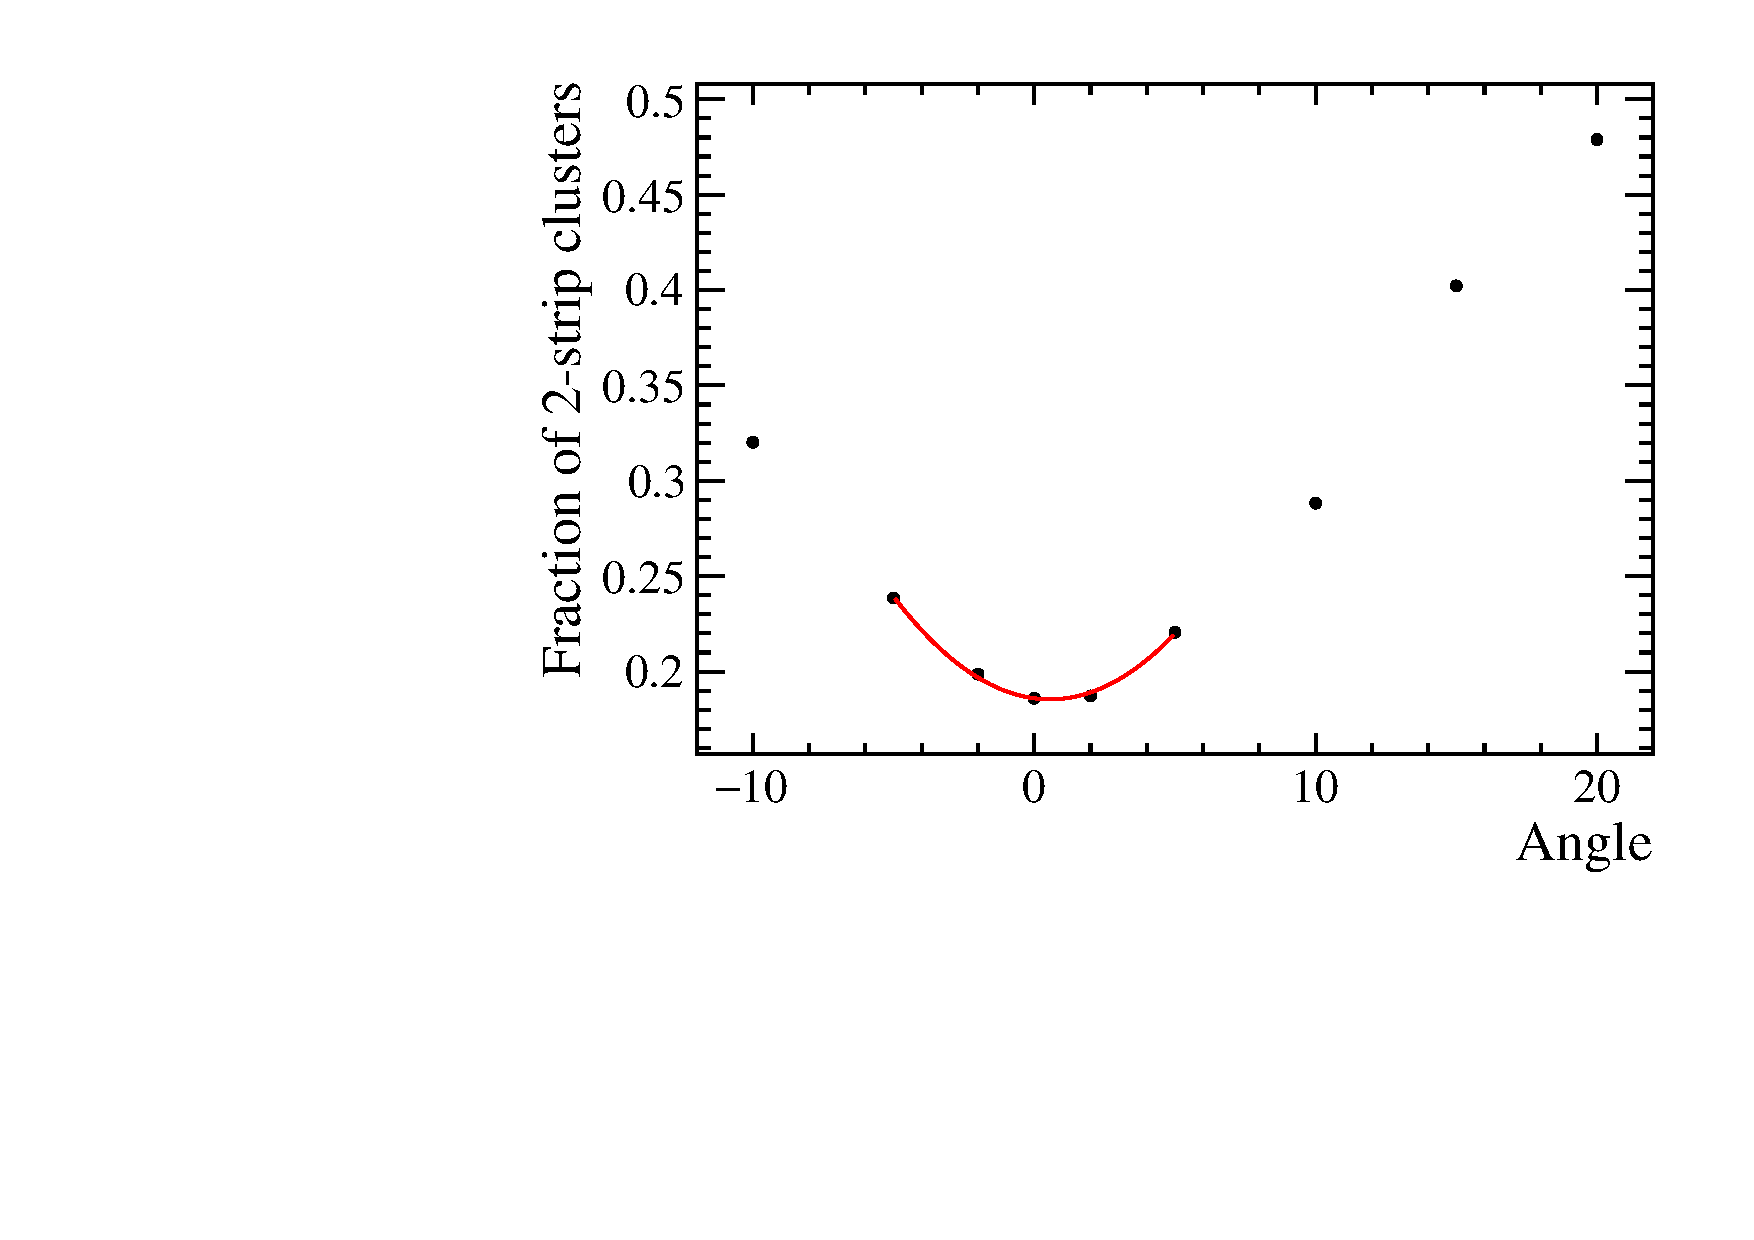
\includegraphics[width=0.45\textwidth]{figs/SNRvsAngle/cf2StripClustervsAngle_M4_FanIn_Top.pdf}
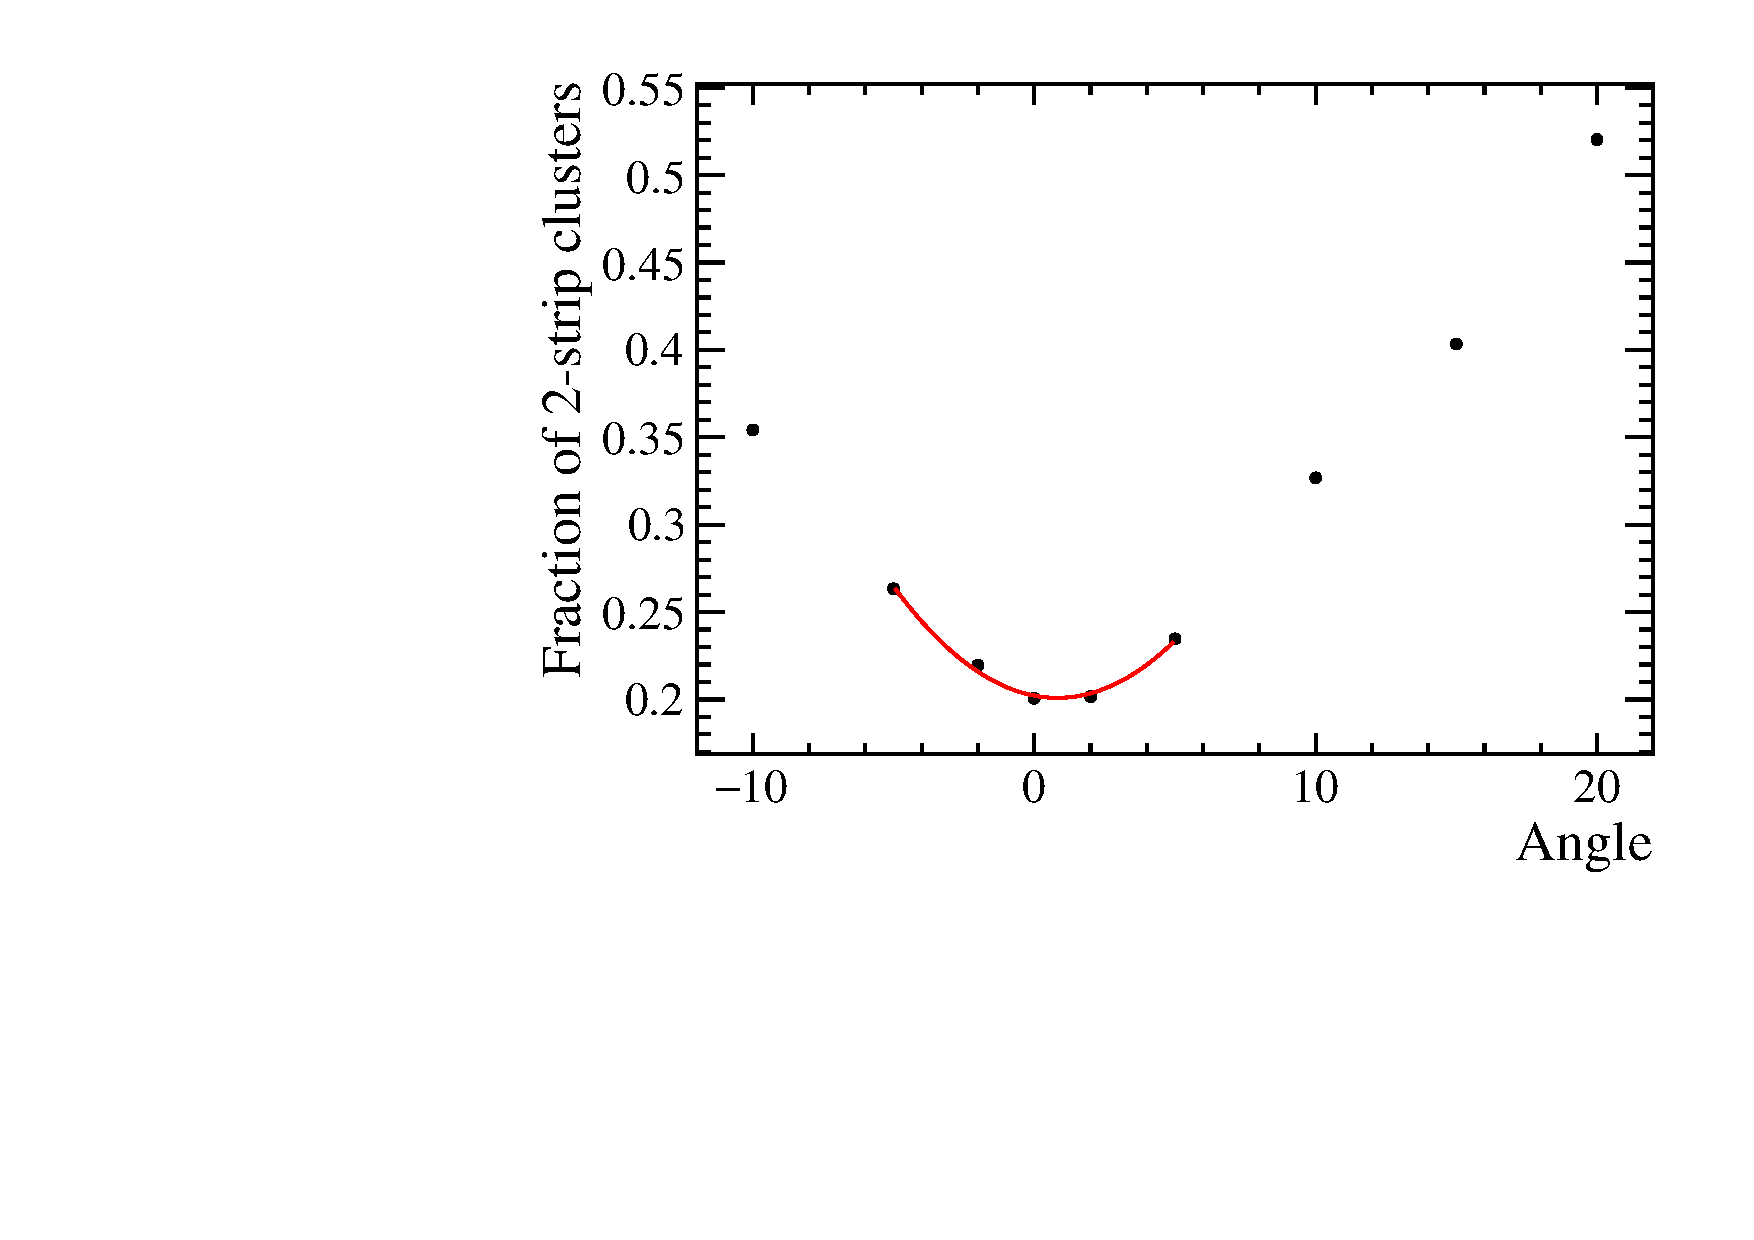
\includegraphics[width=0.45\textwidth]{figs/SNRvsAngle/cf2StripClustervsAngle_M4_FanUp_Top.pdf}
\caption[Fraction of $1$-strip and $2$-strip clusters as a function of the rotation around the $y$ axis.]{Fraction of $1$-strip (top) and $2$-strip (bottom) clusters as a function of the rotation around the $y$ axis for the M4 fan-in (left) and fan-up (right) sensors, both with top biasing.}
\label{fig:fStripClustersvsAngle}
\end{figure}